\documentclass[%
a4paper,
twoside
]{scrreprt}

\usepackage[utf8]{inputenc}
\usepackage[T1]{fontenc}
\usepackage{lmodern}

% \usepackage[bibfile=mybib.bib,bibstyle=authoryear]{cleanthesis}

% \usepackage{natbib}
\usepackage[
  backend=bibtex,
  style=authoryear,
  natbib,
  backref
]{biblatex}

\addbibresource{mybib.bib}

\usepackage{amsmath}
\usepackage{amssymb}
\usepackage{amsfonts}
\usepackage{bm}
\usepackage{float}
\usepackage{graphicx}

\usepackage{tikz}
\usetikzlibrary{arrows,decorations.pathmorphing,backgrounds,positioning,fit,petri,decorations.pathreplacing}
\tikzset{circly/.style={draw,circle,minimum size=1cm},
    arraycell/.style={draw,rectangle,minimum size=1cm,node distance=0},
    accolade/.style={decorate,decoration={brace,amplitude=10pt}},
    enoughdamnvspace/.style={font=\vphantom{$ f $}},
    smallnode/.style={circle,fill,inner sep=0,minimum size=5pt}}

\usepackage{subcaption}
\usepackage{caption} % to remove colon from figures with no caption
% \usepackage[top=3cm, left=2cm, right=2cm, bottom=3cm]{geometry}

\usepackage[%
%colorlinks=false,hidelinks
]{hyperref}
\usepackage{algorithm}
\usepackage{algorithmicx}
\usepackage[noend]{algpseudocode}

\algnewcommand{\LineComment}[1]{\State \(/*\) #1 \(*/\)}

\usepackage{listings}
\usepackage{courier}
\usepackage{amsthm}

\usepackage[gen]{eurosym}

\lstset{basicstyle=\footnotesize\ttfamily,breaklines=true}

\renewcommand{\sfdefault}{phv}
\renewcommand{\rmdefault}{bch}

\newtheoremstyle{mydefinitionstyle} % name of the style to be used
  {10mm}        % measure of space to leave above the theorem. E.g.: 3pt
  {10mm}        % measure of space to leave below the theorem. E.g.: 3pt
  {}            % name of font to use in the body of the theorem
  {2em}  % measure of space to indent
  {\bfseries}   % name of head font
  {.}    % punctuation between head and body
  {10mm}        % space after theorem head
  {}            % Manually specify head

\theoremstyle{definition}
\newtheorem{definition}{Definition}

% \setlength{\parindent}{0em}
% \setlength{\parskip}{0.5em}
% \renewcommand{\baselinestretch}{1.25}

\hyphenation{time-stamp}

\begin{document}

\frenchspacing

\title{Evaluation of Algorithms for Sequential Pattern Mining in Long Event Sequences}
\subtitle{}

%***********************************************************************
% AUTHORS INFORMATION AREA
%***********************************************************************
\author{Josse Coen
\vspace{.3cm}\\
%
% Addresses and institutions (remove "1- " in case of a single institution)
University of Antwerp
%
% Remove the next three lines in case of a single institution
% \vspace{.1cm}\\
% 2- School of Second Author - Dept of Second Author \\
% Address of Second Author's school - Country of Second Author's school\\
}
%***********************************************************************
% END OF AUTHORS INFORMATION AREA
%***********************************************************************

\date{1 January 1970}

% \newcommand*{\plogo}{\fbox{$\mathcal{PL}$}} % Generic publisher logo

%----------------------------------------------------------------------------------------
%   TITLE PAGE
%----------------------------------------------------------------------------------------

\newcommand*{\titleGM}{\begingroup % Create the command for including the title page in the document
\mbox{ % Horizontal box
\hspace*{0.2\textwidth} % Whitespace to the left of the title page
\rule{1pt}{0.95\textheight} % Vertical line
\hspace*{0.05\textwidth} % Whitespace between the vertical line and title page text
\begin{minipage}[b][0.95\textheight][t]{0.75\textwidth} % Paragraph box which restricts text to less than the width of the page

\vspace{0.1\textheight}

{\noindent\Large\bfseries\sffamily Evaluation of Algorithms for Sequential\\Pattern Mining in Long Event Sequences }\\[2\baselineskip] % Title
{\Large Josse Coen}\\[2\baselineskip] % Author name
A dissertation submitted in partial fulfillment of the requirements for the degree of Master in Computer Science: Data Science.\\[2\baselineskip]
{\large Principal supervisor: Prof. Dr. Bart Goethals}\\[0.25\baselineskip]
{\large Assistant supervisor: Dr. Boris Cule}\\[2\baselineskip]
{\large September 2018} \\[2\baselineskip]
{\large {Department of Mathematics and Computer Science  \\[0.25\baselineskip] University of Antwerp}}\\[3\baselineskip]

% \vspace{0.4\textheight} % Whitespace between the title block and the publisher
% {\noindent The Publisher \plogo}\\[\baselineskip] % Publisher and logo
\end{minipage}
}
\endgroup}

\titleGM % This command includes the title page

\tableofcontents
\newpage

% \chapter{Introduction}

In data mining, the goal is generally to extract useful information from datasets that are too large for a person to draw conclusions from without studying the data extensively, without any kind of summarization or other means of processing. Data mining encompasses the analysis of different kinds of data using a variety of methods.

One of the subdomains in data mining is frequent pattern mining. In frequent pattern mining, a large database of transactions --- each transaction consisting of a (relatively small) set of items --- is mined for frequent \emph{itemsets}, that is, sets of items that often co-occur within transactions. A commonly cited use case are supermarket transactions, where each item in a transaction is an item that a customer bought during a visit to the store.

A well-known algorithm for mining itemsets in such a transactional database is Apriori, introduced by \citeauthor{agrawal1994fast} \citep{agrawal1994fast}, which relies on the fact that an itemset cannot be more frequent than any of its subsets, allowing the search space to be pruned heavily. It uses a breadth-first approach --- first finding all 1-sized itemsets, then all 2-sized itemsets, and so on --- generating larger candidates from smaller itemsets that are known to be frequent.

From itemsets that have been found frequent (or otherwise interesting), \emph{association rules}~\cite{agrawal1994fast} are used to find sets of items where the occurrence of one set can be a good predictor of another.

A first exploration into mining patterns in data of a sequential nature still presumed a database of transactions, with (relatively short) sequences as transactions instead of sets \citep{agrawal1995mining}.
Since the data format is similar to that of typical frequent pattern mining, mining algorithms are often similar to those in frequent pattern mining as well.

Later, \citeauthor{mannila1997discovery} introduced a new kind of setting for mining patterns in single, long \emph{sequences} \citep{mannila1997discovery}, where \emph{events} occur at certain points in time.

Such sequences may represent different kinds of data. A few examples:
\begin{itemize}
\item Activity logs: whether or not a pattern of activity is cause for alarm \cite{mannila1997discovery}.
\item Machine logs, where the goal of mining data could be to predict failures beforehand and perform maintenance as needed.
\item Any kind of text: books, articles, tweets, transcripts, \ldots
\item Logs of user behaviour: How does a person use a graphical user interface? What patterns do gamblers exhibit when playing video poker?
\item Biosequences \cite{biosequences}.
\end{itemize}

Though the main goal of finding patterns remains equivalent, the mining techniques used for these kinds of data stray further from those in the transactional setting. In sequential pattern mining, the main bottleneck is the length of the sequence, rather than the number of transactions.

Whereas patterns consist of itemsets in frequent pattern mining, in sequential pattern mining we speak of \emph{episodes}. If one wants to assess the interestingness of an episode by how frequently it appears in the sequence, then the search space can be pruned in much the same way that Apriori does in frequent pattern mining.

In chapter~\ref{sec:problem-statement} we begin by formally defining the structure of the datasets we'll operate on: \emph{event sequences}. Then we will move on to \emph{patterns}: how do we define a pattern on an event sequence?
And how do we quantify how interesting a pattern is in regard to an event sequence?

Then, in chapter~\ref{sec:algorithms} we will present and implement algorithms which mine patterns according to the interestingness measures we defined.

In chapter~\ref{sec:experiments} we experiment to make an assessment of the implementation, in terms of:

\begin{enumerate}
\item the performance: how efficient is the implementation with a variety of datasets and parameters?
\item the quality of the output: can we find interesting patterns in different datasets? How does our implementation compare to other implementations which use other interestingness measures and classes of episodes?
\end{enumerate}

To make such an evaluation, we will use a number of datasets of different kinds, fit them into event sequences, study the runtime of the algorithm across a range of parameters, and judge the quality of the output.


% \chapter{Nederlandse samenvatting}
% \newpage

\section{Problem Statement}

\subsection{Event sequences}

\begin{definition}
A \emph{sequence event}, or \emph{event} for short, is defined as a pair $ (A, t) $ where $ A \in \Sigma $ is an event type from a given set of event types $ \Sigma $, and $ t $ is a timestamp integer.
\end{definition}

\begin{definition}
An \emph{event sequence} $ \boldsymbol{s} $ is a triple $ (s, T_s, T_e) $, where $ s $ is an ordered sequence of events
\begin{align*}
s = \langle (A_1, t_1), (A_2, t_2), \, \ldots, \, (A_n, t_n) \rangle
\end{align*}
such that $ t_i \leq t_{i + 1} $ for all $ i = 1, \, \ldots, \, n - 1 $, and any given pair $ (A, t) $ appears at most once.

With $ \boldsymbol{s}_i $ we refer to the pair $ (A_i, t_i) $ in $ s $.

$ T_s $ and $ T_e $ are timestamps such that $ T_s \leq t_1 $ and $ t_n < T_e $. They mark the beginning and the end of the sequence, respectively.

If a sequence event $ (A, t) $ is in $ s $ for a given sequence $ \boldsymbol{s} $, we say that the event \emph{occurs} in $ \boldsymbol{s} $ at timestamp $ t $.
\end{definition}

Note that multiple events can occur at the same timestamp, if they have different event types. Some implementations do not allow this, however.

\begin{definition}
Given a sequence $ \boldsymbol{s} = (s, T_s, T_e) $ and two timestamps $ t_s $ and $ t_e $,
% such that $ t_s < T_e $ and $ T_s < t_e $
we define a \emph{window} on $ \boldsymbol{s} $ to be an event sequence $ (w, t_s, t_e) $ where $ w $ contains all events $ (A, t) $ in $ s $ where $ t_s \leq t < t_e $.
\end{definition}

Note that in the previous definition, $ t_s $ and $ t_e $ do not have to be within the sequence.

For the sake of simplicity, we use the notation $ s_1 \cdots s_n $ to mean the sequence $ (\langle (s_1, 1), \ldots,\allowbreak(s_n, n) \rangle, 1, n + 1) $.

\begin{figure}
\centering

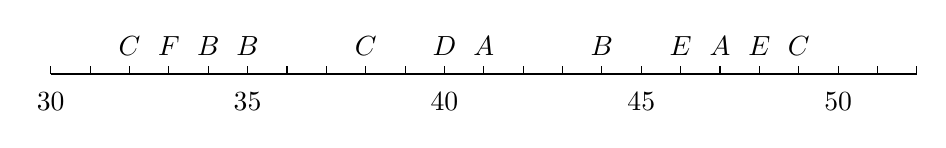
\begin{tikzpicture}

\draw (-5.5,0) -- (5.5,0);

\foreach \x in {-5.5,-5,...,5.5}
    \draw (\x,0) -- (\x,3pt);

\foreach \x [evaluate=\x as \timestamp using int((\x*2)+41)] in {-5.5,-3,...,5.5}
    \node at (\x,-1em) {$ \timestamp $};


\foreach \x/\eventtype in {
  -4.5/C,
  -4/F,
  -3.5/B,
  -3/B,
  -1.5/C,
  -0.5/D,
  -0/A,
  1.5/B,
  2.5/E,
  3/A,
  3.5/E,
  4/C}
    \node at (\x,1em) {$ \eventtype $};

\end{tikzpicture}

\caption{A visual example of a sequence.}

\label{fig:event-sequence}
\end{figure}

Figure~\ref{fig:event-sequence} shows a visualization of a possible event sequence.

\begin{definition}
An \emph{episode} $ \alpha $ is a directed acyclic graph with labelled nodes, that is, $ \alpha = (V, E, lab) $, where $ V = (v_1, \ldots, v_k) $ is the set of nodes, $ E $ is the set of directed edges, and \emph{lab} is a function $ lab \colon V \rightarrow \Sigma $, mapping each node $ v_i $ to an event type. If $ lab(v) = A $, then we say that node $ v $ is of (event) type $ A $.
\end{definition}

We write $ | \alpha | $ to mean the number of nodes in an episode's graph. We call $ | \alpha | $ the \emph{size} of $ \alpha $.

\begin{definition}
A node $ n $ in an episode graph is a \emph{descendant} of a node $ m $ if there is a path from $ m $ to $ n $. Conversely $ m $ is an \emph{ancestor} of $ n $ in that case.
\end{definition}

\begin{definition}
Given a sequence $ s $ and an episode $ G $ we say that $ s $ \emph{covers} G, or $ G $ \emph{occurs} in $ s $, if there is an injective map $ f $ mapping each node $ v_i $ to a valid index such that:
\begin{enumerate}
\item the node $ v_i $ in $ G $ and the corresponding sequence element $ s_{f(v_i)} $ have the same label: $ s_{f(v_i)} = lab(v_i) $, and
\item if there is an edge $ (v_i, v_j) $ in $ G $, then we must have $ f(v_i) < f(v_j) $. In other words, the parents of $ v_j $ must occur in $ s $ before $ v_j $. If the mapping $ f $ is surjective, that is, all events in $ s $ are used, we will say that $ s $ is an \emph{instance} of G.
\end{enumerate}
\end{definition}

\begin{definition}
Given two episodes $ G $ and $ H $, we say that $ G $ is a \emph{subepisode} of $ H $, denoted $ G \subseteq H $, if the set of all sequences that cover $ H $ is a subset of the set of all sequences that cover $ G $. If $ G $ and $ H $ are strict episodes, $ G \subseteq H $ if the graph describing episode $ G $ is a subgraph of the graph describing episode $ H $.
\end{definition}

In this thesis, we'll be limiting ourselves to two subcategories of episodes:
\begin{itemize}
\item \textbf{Parallel episodes.} A parallel episode is an episode for which the set of edges is empty. As such, no constraints are placed on the order in which event types occur in a sequence. An example is shown in figure~\ref{fig:episode-graphs-parallel}. In text we'll write parallel episodes by their event types using the following notation:
\begin{align*}
    \{ A_1, A_2, \ldots, A_n \}
\end{align*}
by which we mean a parallel episode with $ n $ nodes, and the event types are $ A_1 $ through $ A_n $. Note that though the notation reminds strongly of the notation for a mathematical set, it does not represent a set: a parallel episode $ \{ A, A, B, C \} $ is not equivalent to an episode $ \{ A, B, C \} $.

\item \textbf{Serial episodes.} A serial episode is an episode for which the edges cause the nodes to have a total order. That way, in any occurrence of a serial episode in a sequence, the event types appear in the same order. Figure~\ref{fig:episode-graphs-serial} shows an example.

% Sometimes it is useful to describe serial episodes in their strict form, in which there is a direct edge between any two nodes. Figure~\ref{fig:episode-graphs-serial-strict} shows a strict episode which is equivalent to the episode in figure~\ref{fig:episode-graphs-serial}.

While serial episodes have a different graph in this form, their meaning is the same, since they enforce the same order on the occurrence of events in the sequence to satisfy an occurrence of a serial episode.

For serial episodes we will use the notation
\begin{align*}
A_1 \to A_2 \to \cdots \to A_n
\end{align*}
where $ A_i $ is the event type of the $ i $-th node.

\end{itemize}

\begin{figure}
\centering

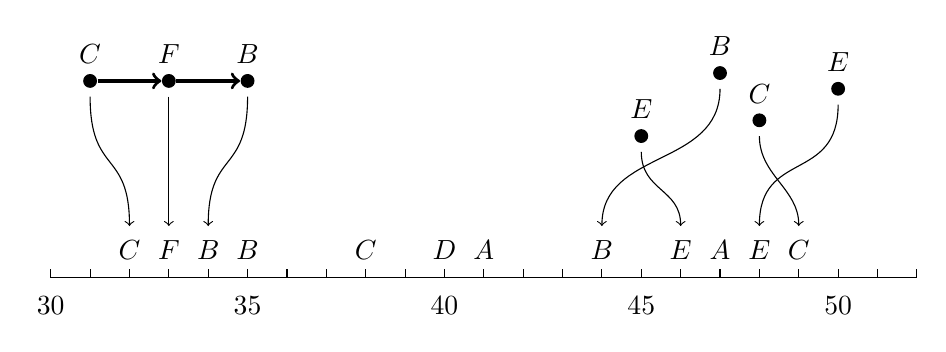
\begin{tikzpicture}[smallnode/.style={circle,fill,inner sep=0,minimum size=5pt}]

\draw (-5.5,0) -- (5.5,0);

\foreach \x in {-5.5,-5,...,5.5}
    \draw (\x,0) -- (\x,3pt);

\foreach \x [evaluate=\x as \timestamp using int((\x*2)+41)] in {-5.5,-3,...,5.5}
    \node at (\x,-1em) {$ \timestamp $};

\foreach \x [evaluate=\x as \timestamp using int((\x*2)+41)] in {-5.5,-5,...,5.5}
    \node (t\timestamp) [inner sep=0] at (\x,1.8em) {};

\foreach \x/\eventtype in {
  -4.5/C,
  -4/F,
  -3.5/B,
  -3/B,
  -1.5/C,
  -0.5/D,
  -0/A,
  1.5/B,
  2.5/E,
  3/A,
  3.5/E,
  4/C}
    \node at (\x,1em) {$ \eventtype $};

% serial episode

\node (serC) at (-5,2.5) [smallnode,label={$ C $}] {};
\node (serF) at (-4,2.5) [smallnode,label={$ F $}] {};
\node (serB) at (-3,2.5) [smallnode,label={$ B $}] {};

\draw [->,very thick] (serC) -- (serF);
\draw [->,very thick] (serF) -- (serB);

\draw [->] ([yshift=-3pt]serC.south) .. controls +(0,-1) and +(0,1) .. (t32);
\draw [->] ([yshift=-3pt]serF.south) .. controls +(0,-1) and +(0,1) .. (t33);
\draw [->] ([yshift=-3pt]serB.south) .. controls +(0,-1) and +(0,1) .. (t34);

% parallel episode

\node (parB) at (3,2.6) [smallnode,label={$ B $}] {};
\node (parE1) at (2,1.8) [smallnode,label={$ E $}] {};
\node (parE2) at (4.5,2.4) [smallnode,label={$ E $}] {};
\node (parC) at (3.5,2) [smallnode,label={$ C $}] {};

\draw [->] ([yshift=-3pt]parB.south) .. controls +(0,-1) and +(0,1) .. (t44);
\draw [->] ([yshift=-3pt]parE1.south) .. controls +(0,-0.5) and +(0,0.5) .. (t46);
\draw [->] ([yshift=-3pt]parE2.south) .. controls +(0,-1) and +(0,1) .. (t48);
\draw [->] ([yshift=-3pt]parC.south) .. controls +(0,-0.5) and +(0,0.5) .. (t49);

\end{tikzpicture}

\caption{Showing an occurrence of a serial episode $ C \to F \to B $ and an occurrence of a parallel episode $ \{ B, C, E, E \} $ in the sequence of figure~\ref{fig:event-sequence}.}
\label{fig:occurrences}
\end{figure}

\begin{figure}

\begin{subfigure}[b]{\textwidth}
\centering
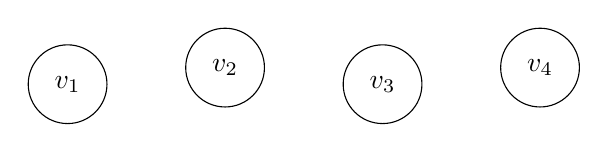
\begin{tikzpicture}

\node (n 1) [circly] at (-3,-3pt) {$ v_1 $};
\node (n 2) [circly] at (-1, 3pt) {$ v_2 $};
\node (n 3) [circly] at ( 1,-3pt) {$ v_3 $};
\node (n 4) [circly] at ( 3, 3pt) {$ v_4 $};

\end{tikzpicture}
\caption{parallel}
\label{fig:episode-graphs-parallel}
\end{subfigure}

\par\bigskip

\begin{subfigure}[b]{\textwidth}
\centering
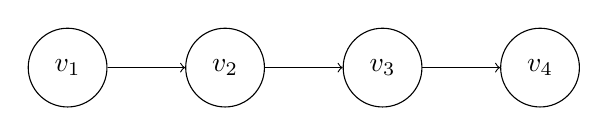
\begin{tikzpicture}

\node (n 1) [circly] at (-3,0) {$ v_1 $};
\node (n 2) [circly] at (-1,0) {$ v_2 $};
\node (n 3) [circly] at ( 1,0) {$ v_3 $};
\node (n 4) [circly] at ( 3,0) {$ v_4 $};

\draw [->] (n 1) -- (n 2);
\draw [->] (n 2) -- (n 3);
\draw [->] (n 3) -- (n 4);

\end{tikzpicture}
\caption{serial}
\label{fig:episode-graphs-serial}
\end{subfigure}

\par\bigskip

\iffalse
\begin{subfigure}[b]{\textwidth}
\centering
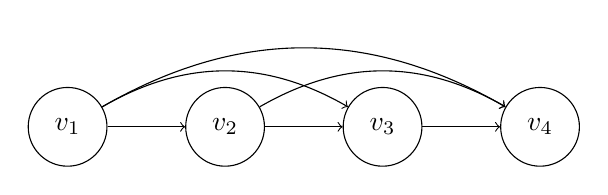
\begin{tikzpicture}

\node (n 1) [circly] at (-3,0) {$ v_1 $};
\node (n 2) [circly] at (-1,0) {$ v_2 $};
\node (n 3) [circly] at ( 1,0) {$ v_3 $};
\node (n 4) [circly] at ( 3,0) {$ v_4 $};

\draw [->] (n 1) -- (n 2);
\draw [->] (n 2) -- (n 3);
\draw [->] (n 3) -- (n 4);

\draw [->] (n 1) to [bend left=30] (n 3);
\draw [->] (n 2) to [bend left=30] (n 4);
\draw [->] (n 1) to [bend left=30] (n 4);

\end{tikzpicture}

\caption{serial, strict}
\label{fig:episode-graphs-serial-strict}
\end{subfigure}
\fi

\caption{Episode graphs.}

\label{fig:episode-graphs}
\end{figure}

Because we only consider parallel and serial episodes, it is easy to represent an episode in a data structure---we don't need to explicitly store a graph with nodes and edges:
\begin{itemize}
\item Parallel episodes can be stored in an array, where each element is simply the event type of the episode. Strictly speaking, the order of the elements in the array doesn't matter, but in the implementation they will follow some order on the set of event types. In that way each parallel episode has a unique array representation. Figure~\ref{fig:parallel-representation} shows the representation visually.

\tikzset{circly/.style={draw,circle,minimum size=1cm},
    arraycell/.style={draw,rectangle,minimum size=1cm,node distance=0}}

\begin{figure}[h]
\centering

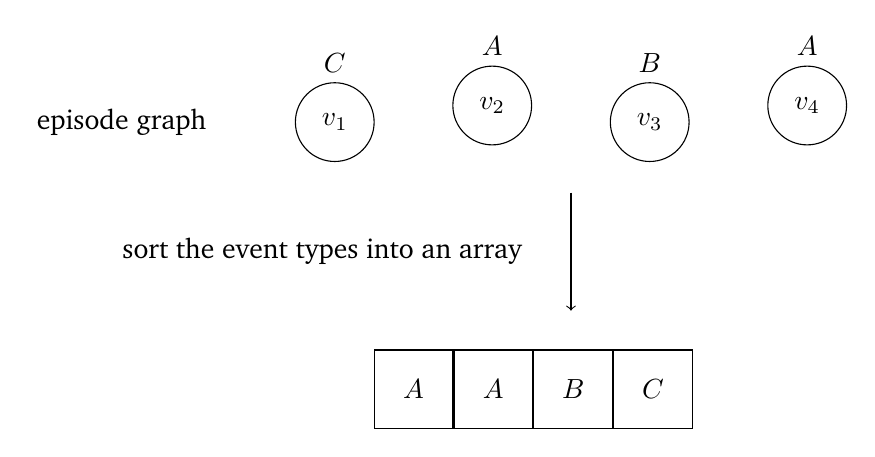
\begin{tikzpicture}

\node (n 1) [circly,label=above:$ C $] at (-3,-3pt) {$ v_1 $};
\node (n 2) [circly,label=above:$ A $] at (-1, 3pt) {$ v_2 $};
\node (n 3) [circly,label=above:$ B $] at ( 1,-3pt) {$ v_3 $};
\node (n 4) [circly,label=above:$ A $] at ( 3, 3pt) {$ v_4 $};

\node [left=of n 1] {episode graph};

\draw [->] (0,-1) -- node [left=0.5cm] {sort the event types into an array} +(0,-1.5);

\node (a 1) [arraycell] at (-2,-3.5) {$ A $};
\node (a 2) [arraycell,right=of a 1] {$ A $};
\node (a 3) [arraycell,right=of a 2] {$ B $};
\node (a 4) [arraycell,right=of a 3] {$ C $};

\end{tikzpicture}

\caption{A parallel episode's graph representation, with the label of each node shown above, and its array representation.}

\label{fig:parallel-representation}
\end{figure}

\item Serial episodes can also be stored in an array, but here the order of the elements is defined by the edges of the episode. That is, the event types are ordered according to a topological sort of the nodes. Figure~\ref{fig:serial-representation} shows this visually.
\end{itemize}

When discussing the algorithms we will mostly consider their array representation, and address the $ i $-th element of an episode array $ \alpha $ with $ \alpha [i] $.

\begin{figure}
\centering

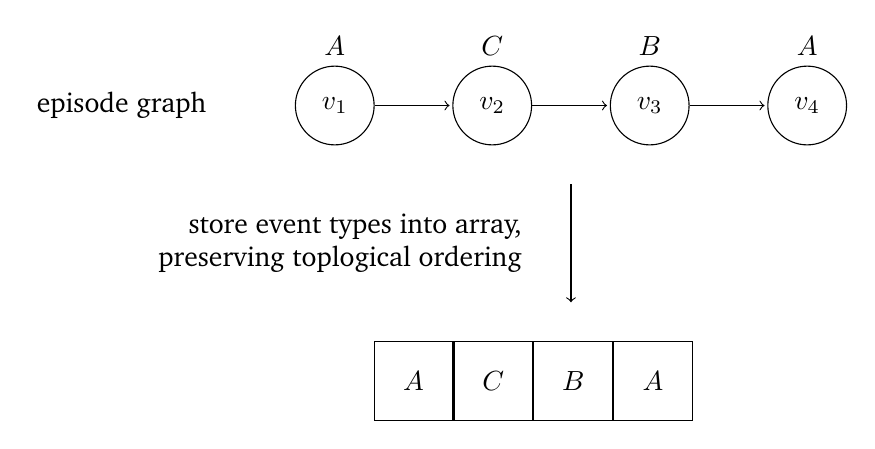
\begin{tikzpicture}

\node (n 1) [circly,label=above:$ A $] at (-3,0) {$ v_1 $};
\node (n 2) [circly,label=above:$ C $] at (-1,0) {$ v_2 $}
    edge [pre] (n 1);
\node (n 3) [circly,label=above:$ B $] at (1, 0) {$ v_3 $}
    edge [pre] (n 2);
\node (n 4) [circly,label=above:$ A $] at (3, 0) {$ v_4 $}
    edge [pre] (n 3);

\node [left=of n 1] {episode graph};

\draw [->] (0,-1) -- node [left=0.5cm,align=right] {store event types into array,\\preserving toplogical ordering} +(0,-1.5);

\node (a 1) [arraycell] at (-2, -3.5) {$ A $};
\node (a 2) [arraycell,right=of a 1] {$ C $};
\node (a 3) [arraycell,right=of a 2] {$ B $};
\node (a 4) [arraycell,right=of a 3] {$ A $};

\end{tikzpicture}

\caption{A serial episode's graph representation, with the label of each node shown above, and its array representation.}
\label{fig:serial-representation}
\end{figure}

\begin{definition}
Given two episodes $ G $ and $ H $ such that $ G \subset H $, we can express an \emph{association rule} $ G \Rightarrow H $. We call $ G $ the \emph{head} of the rule, and $ H $ the \emph{tail} of the rule.
\end{definition}

\subsection{Frequency measures}

We present three methods to measure the frequency of an episode and the confidence of an association rule. In a later section, we implement a mining algorithm based on them.

\subsubsection{Fixed windows}

The first frequency measure is based on windows of fixed length.

\begin{definition}
Given a window size $ \rho $ and a sequence $ s $, we define the \emph{fixed-window frequency} of an episode $ G $ in $ s $, denoted $ fr_f(G; s) $, to be the number of windows of size $ \rho $ in $ s $ covering the episode:
\begin{align*}
fr_f(G; s) = | \{ s[i, i + \rho - 1] | s[i, i + \rho - 1] \text{ covers } G \} |
\end{align*}
\end{definition}

\begin{definition}
Given a window size $ \rho $ and episodes $ X $ and $ Y $, such that $ X \subset Y $, we define the \emph{fixed-window confidence} of the association rule $ X \Rightarrow Y $, denoted $ c_f(X \Rightarrow Y) $, to be the ratio of their respective frequencies:
\begin{align*}
c_f(X \Rightarrow Y) = \frac{ fr_f(Y) }{ fr_f(X) }
\end{align*}
\end{definition}

\subsubsection{Minimal windows}

\begin{definition}
Given a sequence $ s $ and an episode $ G $, a window $ s[a, b] $, is called a \emph{minimal window} of $ G $ in $ s $, if:
\begin{itemize}
\item $ len(s[a, b]) \leq \rho $, $ s[a, b] $, and
\item no proper subwindow of of $ s[a, b] $ covers $ G $.
\end{itemize}
We define beginning, end ... % TODO figure out definitions (inclusive-exclusive end-timestamp)

We denote the set of all minimal windows of $ G $ in $ s $ with $ mw(G; s) $, or simply $ mw(G) $ if $ s $ is known from the context. Given a set of minimal windows $ W $, we define a function $ dis(W) $ to be equal to 1 if all windows in $ W $ are pairwise disjoint, and 0 otherwise.
\end{definition}

\begin{definition}
The \emph{disjoint-window frequency} of an episode $ G $ in a sequence $ s $, denoted $ fr_m(G) $, is defined as the maximal number of non-overlapping minimal windows within $ s $ that contain episode $ G $. Formally:
\begin{align*}
fr_m(G) = \text{max} \{ | W | \mid W \subseteq mw(G) \wedge dis(W) = 1 \}
\end{align*}
\end{definition}

\begin{definition}
Given episodes $ X $ and $ Y $, such that $ X \subset Y $, and a minimal window $ s[a, b] $ of episode $ X $. Assume there exists a minimal window $ s[c, d] $ of $ Y $ such that $ c \leq a $ and $ b \leq d $, then we define the \emph{minimal-extensibility} of occurrence $ s[a, b] $ of $ X $ into an occurrence of $ Y $ as
\begin{align*}
ext_m(s[a, b], X, Y) = 1
\end{align*}
If there exists no such minimal window of $ Y $, we define $ ext_m(s[a, b], X, Y) = 0 $.
\end{definition}

\subsubsection{Weighted minimal windows}

\begin{definition}
The \emph{total weight} of a set of windows $ W $ in a sequence $ s $, denoted $ tw(W) $, is defined as
\begin{align*}
tw(W) = \sum_{w \in W}{\frac{1}{len(w)}}
\end{align*}
The \emph{weighted-window frequency} of an episode $ G $ in a sequence $ s $, denoted $ fr_w(G) $, is defined as
\begin{align*}
fr_w(G) = \text{max} \{ tw(W) | W \subseteq mw(G), dis(W) = 1 \}
\end{align*}
\end{definition}

\subsection{Other interestingness measures}

\newpage


\section{Algorithms}

\subsection{Finding frequent episodes: high-level algorithm}

\begin{algorithm}

\caption{High-level algorithm for finding frequent episodes. \\
Input: A set $ \Sigma $ of event types, an event sequence $ s $ over $ \Sigma $, a window width \emph{win}, and a frequency threshold \emph{min\_fr}. \\
Output: The collection of episodes that are frequent in the sequence in terms of the input parameters.
}

\begin{algorithmic}[1]

\State $ \mathcal{C}_1 \gets \Sigma $
\State $ l \gets 1 $
\While{$ \mathcal{C}_l \neq \emptyset $}
    \LineComment{Database pass (algorithms \ref{alg:rec-par-fwi}, \ref{alg:rec-ser-fwi}, ...)}
    \State compute $ \mathcal{F}_l \gets \{ \alpha \in \mathcal{C}_l \mid fr(\alpha, s, \text{win}) \geq \text{min\_fr} \} $
    \State $ l \gets l + 1 $
    \LineComment{Candidate generation (algorithm \ref{alg:cand-gen})}
    \State compute $ C_l = \{ \alpha \mid | \alpha | = l \wedge \forall \beta \mid \beta \subset \alpha : \beta \text{ is frequent} \} $
\EndWhile
\State output all $ \mathcal{F}_i $

\end{algorithmic}

\label{alg:episodes-top-level}
\end{algorithm}

% TODO Read this future me, probably needs improvement.

Algorithm~\ref{alg:episodes-top-level} describes the high-level procedure to find all frequent episodes of a certain class (parallel or serial) that are frequent in an event sequence $ s $, given window width \emph{win} and frequency threshold \emph{min\_fr}. It is a breadth-first algorithm, that is, all frequent episodes of size $ l $ are computed before those of size $ l + 1 $.

The construction of the first set of candidates is a special case. $ \mathcal{C}_1 $ consists of simply all possible episodes with one node. That's one episode per event type, and so $ | C_1 | = | \Sigma | $. After constructing $ \mathcal{C}_1 $ a loop is entered where
ever-bigger episodes are constructed and filtered by frequency in the sequence.
% for each $ l $, it is determined which episodes are frequent ($ \mathcal{F}_1 $), by a pass over the sequence, and subsequently, based on those, candidates of size $ 2 $ are generated. The loop continues with ever-increasing episode size $ l $, and stops when no more candidates were generated. Then all frequent episodes have been found.

The following subsections will cover all of the subalgorithms.

\subsection{Candidate generation}
\label{sec:cand-gen}

\begin{algorithm}

\caption{Generating candidate parallel episodes of size $ l + 1 $ from frequent parallel episodes of size $ l $. \\
Input: A sorted array $ \mathcal{F}_l $ of frequent parallel episodes of size $ l $. \\
Output: A sorted array of candidate parallel episodes of size $ l + 1 $.
}

\begin{algorithmic}[1]

\State $ \mathcal{C}_{l + 1} \gets \emptyset $
\State $ k \gets 0 $
\If{$ l = 1 $}
    \For{$ h \gets 1 $ to $ | \mathcal{F}_l | $} $ \mathcal{F}_l \text{.block\_start}[h] \gets 1 $ \EndFor
\EndIf
\For{$ i \gets 1 $ to $ | \mathcal{F}_l | $} \label{alglin:cand-gen:i-loop}
    \State $ \text{current\_block\_start} \gets k + 1 $
    \For{$ j \gets i $; $ \mathcal{F}_l \text{.block\_start}[j] = \mathcal{F}_l \text{.block\_start}[i] $; $ j \gets j + 1 $}
    \label{alglin:cand-gen:j-loop}
        \LineComment{$ \mathcal{F}_l[i] $ and $ \mathcal{F}_l[j] $ have $ l - 1 $ first event types in common, build a potential candidate $ \alpha $ as their combination.}
        \For{$ x \gets 1 $ to $ l $} $ \alpha[x] \gets \mathcal{F}_l[i][x] $ \label{alglin:cand-gen:construct-candidate-1}
        \EndFor
        \State $ \alpha[l + 1] \gets \mathcal{F}_l[j][l] $ \label{alglin:cand-gen:construct-candidate-2}
        \LineComment{Build and test subepisodes $ \beta $ that do not contain $ \alpha[y] $}
        \For{$ y \gets 1 $ to $ l - 1 $} \label{alglin:cand-gen:test-subepisodes-loop}
            \For{$ x \gets 1 $ to $ y - 1 $} $ \beta[x] \gets \alpha[y] $
            \EndFor
            \For{$ x \gets y $ to $ l $} $ \beta[x] \gets \alpha[x + 1] $
            \EndFor
            \If{$ \beta $ is not in $ \mathcal{F}_l} $ continue with the next $ j $ at line~\ref{alglin:cand-gen:j-loop}
            \EndIf
        \EndFor
        \LineComment{All subepisodes are in $ \mathcal{F}_l $, store $ \alpha $ as candidate}
        \State $ k \gets k + 1 $
        \State $ \mathcal{C}_{l + 1}[k] \gets \alpha $
        \State $ \mathcal{C}_{l + 1} \text{.block\_start}[k] \gets \text{current\_block\_start} $
    \EndFor
\EndFor
\State output $ \mathcal{C}_{l + 1} $

\end{algorithmic}

\label{alg:cand-gen}
\end{algorithm}

% TODO show modification for serial episodes

Algorithm~\ref{alg:cand-gen} generates candidates of size $ l + 1 $ from a collection of frequent parallel episodes of size $ l $. It can be easily modified to generate serial episodes, as we'll show later in this subsection. Thanks to the monotonic property of the frequency measures we implement, some candidates can be immediately proven infrequent. More specifically, if there exists an infrequent subepisode $ \beta $ of candidate $ \alpha $, then $ \alpha $ is not frequent.
Conveniently, all frequent subepisodes of size $ l $ are already given as input to the algorithm. So when the algorithm constructs a candidate of size $ l + 1 $, all of its subepisodes of size $ l $ are checked to be frequent by testing whether they are in the input collection $ \mathcal{F}_l $. If one of the subepisodes is not in $ \mathcal{F}_l $, then it is infrequent and, consequently, the potential candidate cannot be frequent either.
Subepisodes smaller than $ l $ do not need to be checked anymore, because any less-than-$ l $-sized subepisode of the potential candidate is also a subepisode of one of the $ l $-sized subepisodes and any $ l $-sized subepisodes that have turned out to be frequent are already known to have frequent subepisodes.

% Combine this paragraph with the one about parallel episode candidate generation?
Parallel episodes are constructed such that the elements in their arrays are sorted according to event type. In this way, a parallel episode has a unique array representation.

Potential candidates of size $ l + 1 $ are generated by combining frequent episodes of size $ l $ which share a prefix of $ l - 1 $ elements. In other words, they are only allowed to differ in their last element. The newly constructed candidate shares these $ l - 1 $ as well, and is then followed by the last elements of both $ \alpha $ and $ \beta $. This method of candidate generation is similar to the way in which candidate itemsets are generated in the Apriori \cite{apriori97} algorithm. Lines~\ref{alglin:cand-gen:construct-candidate-1} and \ref{alglin:cand-gen:construct-candidate-2} implement this. Figure~\ref{fig:parallel-episode-combined} shows an example of two episodes being combined, and figure~\ref{fig:parallel-episode-lattice} shows visually how larger candidates build upon smaller episodes.

\begin{figure}
\centering

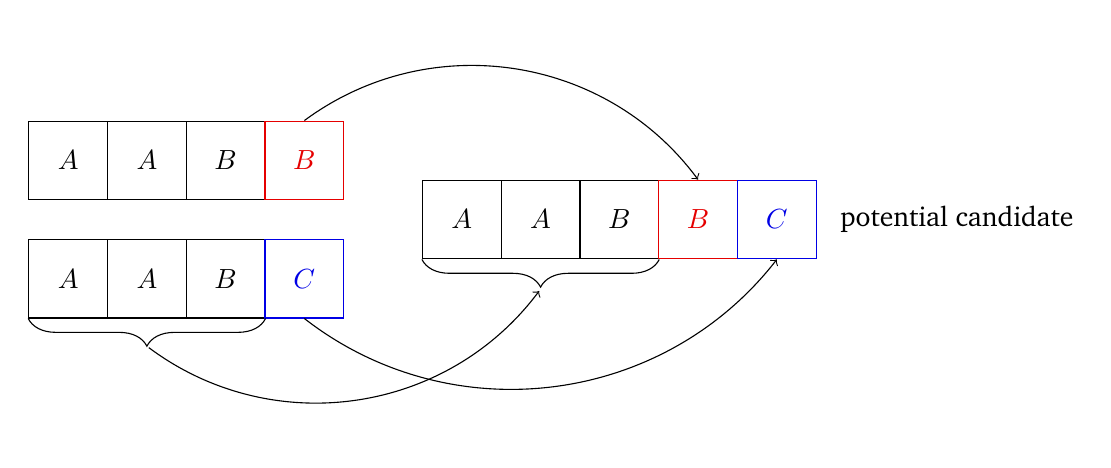
\begin{tikzpicture}

\newcommand\sharedprefix[1]
{
    \ifcase#1 A
    \or A
    \or B
    \fi
}

\foreach \arrayindex [evaluate=\arrayindex as \leftx using int(\arrayindex-4),
                      evaluate=\arrayindex as \rightx using (int(\arrayindex+1))] in {0,...,2}
{
    \node (n\arrayindex0) [arraycell] at (\leftx,0.75) {$ \sharedprefix{\arrayindex} $};
    \node (n\arrayindex1) [arraycell] at (\leftx,-0.75) {$ \sharedprefix{\arrayindex} $};
    \node (n\arrayindex2) [arraycell] at (\rightx,0) {$ \sharedprefix{\arrayindex} $};
}

\node (n30) [arraycell,color=red!90!black] at (-1,0.75) {$ B $};
\node (n31) [arraycell,color=blue!90!black] at (-1,-0.75) {$ C $};

\node (n32) [arraycell,color=red!90!black] at (4,0) {$ B $};
\node (n42) [arraycell,color=blue!90!black] at (5,0) {$ C $};

\draw [->] (n30.north) to [bend left=45] (n32.north);
\draw [->] (n31.south) to [bend right=45] (n42.south);

\draw [accolade] (n21.south east) -- node (acc1tip) [inner sep=0,midway,yshift=-10pt] {} (n01.south west);
\draw [accolade] (n22.south east) -- node (acc2tip) [inner sep=0,midway,below,yshift=-10pt] {} (n02.south west);

\draw [->] (acc1tip) to [bend right=45] (acc2tip);

% \node [above=of n00] {first episode};
% \node [below=of n01] {second episode};

\node [right=5pt of n42] {potential candidate};

\end{tikzpicture}

\caption{Two episodes being combined into a larger episode.}
\label{fig:parallel-episode-combined}
\end{figure}

\begin{figure}
\centering

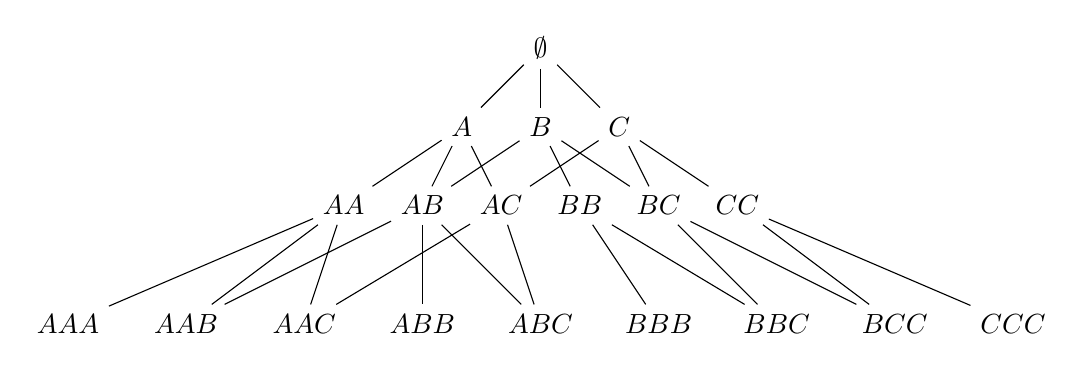
\begin{tikzpicture}

\node (e) at (0,0) {$ \emptyset $};
\node (A) at (-1,-1) {$ A $};
\node (B) at (0,-1) {$ B $};
\node (C) at (1, -1) {$ C $};

\node (AA) at (-2.5,-2) {$ AA $};
\node (AB) at (-1.5,-2) {$ AB $};
\node (AC) at (-0.5,-2) {$ AC $};
\node (BB) at (0.5,-2) {$ BB $};
\node (BC) at (1.5,-2) {$ BC $};
\node (CC) at (2.5,-2) {$ CC $};

\node (AAA) at (-6,-3.5) {$ AAA $};
\node (AAB) at (-4.5,-3.5) {$ AAB $};
\node (AAC) at (-3,-3.5) {$ AAC $};
\node (ABB) at (-1.5,-3.5) {$ ABB $};
\node (ABC) at (0,-3.5) {$ ABC $};
\node (BBB) at (1.5,-3.5) {$ BBB $};
\node (BBC) at (3,-3.5) {$ BBC $};
\node (BCC) at (4.5,-3.5) {$ BCC $};
\node (CCC) at (6,-3.5) {$ CCC $};

\draw (e) -- (A);
\draw (e) -- (B);
\draw (e) -- (C);

\draw (A) -- (AA);
\draw (A) -- (AB);
\draw (B) -- (AB);
\draw (A) -- (AC);
\draw (C) -- (AC);
\draw (B) -- (BB);
\draw (B) -- (BC);
\draw (C) -- (BC);
\draw (C) -- (CC);

\draw (AA) -- (AAA);
\draw (AA) -- (AAB);
\draw (AB) -- (AAB);
\draw (AB) -- (ABB);
\draw (AA) -- (AAC);
\draw (AC) -- (AAC);
\draw (AB) -- (ABC);
\draw (AC) -- (ABC);
\draw (BB) -- (BBB);
\draw (BB) -- (BBC);
\draw (BC) -- (BBC);
\draw (BC) -- (BCC);
\draw (CC) -- (BCC);
\draw (CC) -- (CCC);

\end{tikzpicture}

\caption{Parallel episode construction for $ \Sigma = \{ A, B, C \} $ up to size 3.}

\label{fig:parallel-episode-lattice}
\end{figure}

The algorithm assumes that the input array of frequent $ l $-sized episodes $ \mathcal{F}_l $ is sorted lexicographically. That is, in the first place the episodes are sorted by the first event type in the array, secondarily by the second element, and so on. The algorithm constructs new episodes in such a way that the output is also ordered lexicographically, and since the ordering is preserved when filtering episodes, the assumption about the input is always true.

As mentioned previously, a potential candidate is generated from two episodes that share an $ (l - 1) $-prefix in their array representation. And with the episodes being ordered as described, all of the episodes that share a prefix are grouped together. As a result, episodes can be grouped into \emph{blocks}, where all of the episodes in a block share the first $ l - 1 $ elements. Then all episodes within the same block are combined. Figure~\ref{fig:blocks} illustrates the block structure.

\newcommand\blockspicvalue[2]{
    \ifcase#2
        \ifcase#1 A
            \or A
            \or B
        \fi
        \or \ifcase#1 A
            \or A
            \or C
        \fi
        \or \ifcase#1 A
            \or C
            \or C
        \fi
        \or \ifcase#1 A
            \or C
            \or D
        \fi
        \or B
        \or \ifcase#1 B
            \or B
            \or C
        \fi
        \or \ifcase#1 B
            \or B
            \or D
        \fi
        \or C
    \fi
}

\begin{figure}
\centering

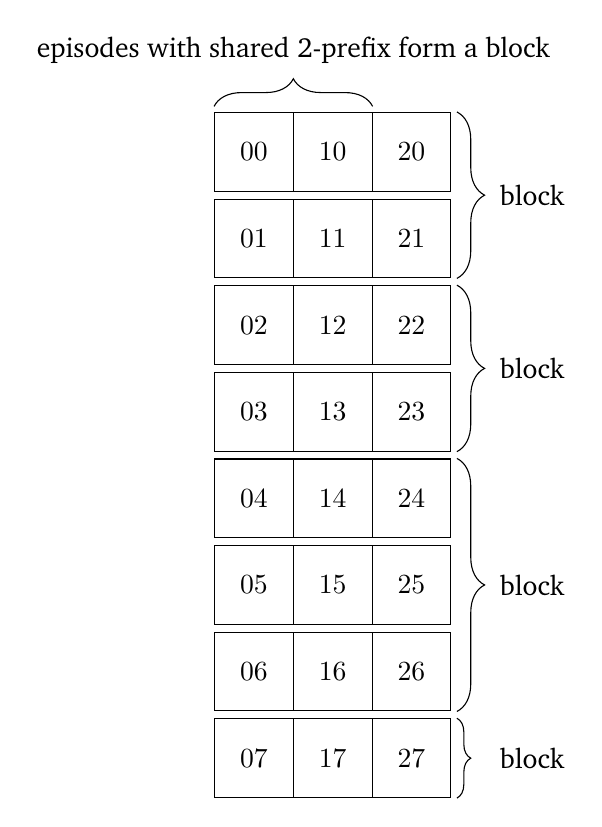
\begin{tikzpicture}

\foreach \x in {0,...,2}
\foreach \y in {0,...,7}
{
    \node (n\x\y) [draw,minimum size=1cm] at (\x,-\y*1.1) {$ \blockspicvalue{\x}{\y} $};
}

\draw[accolade]([yshift=2pt]n00.north west) -- ([yshift=2pt]n10.north east) node [midway,above=12pt] {episodes with shared 2-prefix form a block};

\draw [accolade] ([xshift=2pt]n20.north east) -- ([xshift=2pt]n21.south east) node [midway,right=12pt] {block};
\draw [accolade] ([xshift=2pt]n22.north east) -- ([xshift=2pt]n23.south east) node [midway,right=12pt] {block};
\draw [accolade] ([xshift=2pt]n24.north east) -- ([xshift=2pt]n26.south east) node [midway,right=12pt] {block};
\draw [decorate,decoration={brace,amplitude=5pt}] ([xshift=2pt]n27.north east) -- ([xshift=2pt]n27.south east) node [midway,right=12pt] {block};

\end{tikzpicture}

\caption{Blocks in candidate generation algorithm with parallel episodes of size 3.}

\label{fig:blocks}
\end{figure}

The block structure is represented as follows.
Each episode $ \alpha $ is associated with a value \emph{block\_start}, which is the array index of the first episode in the block which contains $ \alpha $, so it points ``back'' to the beginning of the block. The first episode in each block points to itself. In this way, it can be easily tested whether two episodes belong to the same block. Figure~\ref{fig:block-values} shows this representation for the episodes in figure~\ref{fig:blocks}.

\begin{figure}
\centering

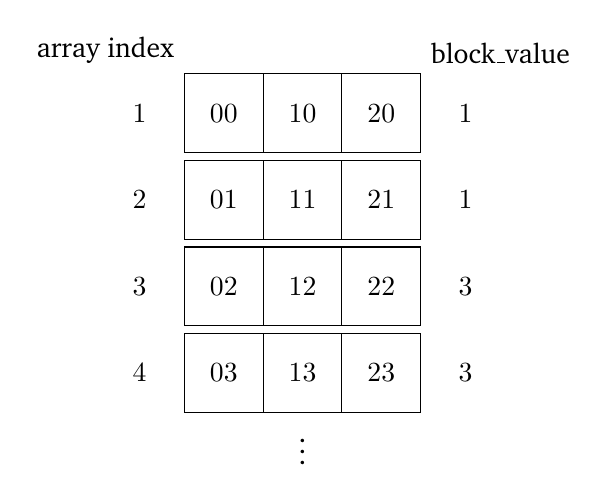
\begin{tikzpicture}

\newcommand\blockspicvaluevalue[1]
{
    \ifcase#1 1
    \or 1
    \or 3
    \or 3
    \fi
}

\foreach \y [evaluate=\y as \arrayindex using int(\y+1)] in {0,...,3}
{
    \foreach \x in {0,...,2}
    {
        \node (n\x\y) [draw,minimum size=1cm] at (\x,-\y*1.1) {$ \blockspicvalue{\x}{\y} $};
    }
    \node [left=10pt of n0\y] {$ \arrayindex $};
    \node [right=10pt of n2\y] {$ \blockspicvaluevalue{\y} $};
}

\node [above left=0 of n00] {array index};
\node [above right=0 of n20] {block\_value};
\node [below=0 of n13] {$ \vdots $};

\end{tikzpicture}

\caption{How blocks are represented in the candidate generation algorithm.}
\label{fig:block-values}
\end{figure}

The algorithm constructs this block structure while generating candidates of size $ l + 1 $, but it also uses the blocks of the $ l $-sized episodes given as input. So it is important that they are preserved and maintained in between different runs of algorithm~\ref{alg:cand-gen}. Section~\ref{sec:maintain-blocks} goes into more detail about this.

We mentioned earlier that in the array representation of parallel episodes, elements are sorted according to event type. We would like to construct parallel candidates for which this is the case as well. We know that the input array of frequent episodes is sorted. Consequently, for any two episodes $ \mathcal{C}[i] $ and $ \mathcal{C}[j] $ in a block such that $ i \leq j $, it holds that $ \mathcal{C}[i][l] \leq \mathcal{C}[j][l] $.
Now, if we always construct a new candidate $ \alpha $ as $ \langle \mathcal{C}[i][1], \ldots,\allowbreak\mathcal{C}[i][l],\allowbreak\mathcal{C}[j][l] \rangle $ and choose $ i $ and $ j $ such that $ i \leq j $, then $ \alpha $'s array representation is sorted by construction. This explains the nested-loop structure of the algorithm (lines~\ref{alglin:cand-gen:i-loop} and~\ref{alglin:cand-gen:j-loop}), where the inner array index $ j $ is always greater than or equal to the outer index $ i $.

With serial episodes on the other hand, the order of elements in the array is not bound by an order on the event types.
Serial candidate generation can be accomplished by a small change to the algorithm. Line~\ref{alglin:cand-gen:j-loop} needs to be changed to:
\begin{algorithmic}[0]
\For{$ j \gets \mathcal{F}_l. \text{block\_start}[i] $; $ \mathcal{F}_l \text{.block\_start}[j] = \mathcal{F}_l \text{.block\_start}[i] $; $ j \gets j + 1 $}
\EndFor
\end{algorithmic}
By initializing $ j $ to $ \mathcal{F}_l \text{.block\_start}[i] $, now $ j $ can be less than $ i $, alleviating the constraint on parallel episodes.

After constructing a potential candidate (lines~\ref{alglin:cand-gen:construct-candidate-1} and \ref{alglin:cand-gen:construct-candidate-2}), it needs to be checked whether all of its subepisodes are frequent.
Constructing all $ l $-sized subepisodes of an $ (l + 1) $-sized candidate $ \alpha $ is straightforward. For each subepisode, one node from $ \alpha $'s graph is left out, until all nodes have been left out. For serial episodes, the edges of the subepisode are constructed such that the order of the toplogical sort is preserved. If we consider the strict form of a serial candidate, an $ l $-sized subepisode can be obtained by leaving one node $ v $ and all edges that contain $ v $. For the array representation of both classes of episodes, this means that one element of the array is left out. See figure~\ref{fig:cand-subepisodes} for an example. In the algorithm, this happens at lines~\ref{alglin:cand-gen:test-subepisodes-loop} and further. The variable $ y $ denotes the array index of the array element that will be left out.

For any potential candidate, two of subepisodes in particular are already known to be frequent, namely the episodes it was built from. Those subepisodes are obtained by leaving out the last and the second to last array elements. That's why the largest value $ y $ takes in the algorithm is $ l - 1 $.

We should note that in the subepisode construction procedure described above, some of the subepisodes may be equivalent to each other, when an event type occurs multiple times in a candidate. For $ \{ A, A, B \} $, subepisode $ \{ A, B \} $ will be constructed twice.

\begin{figure}
\centering

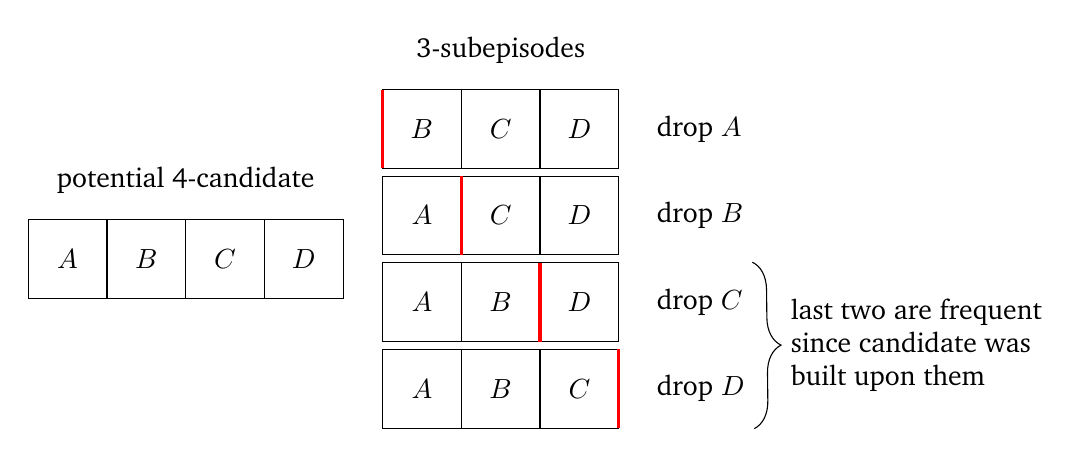
\begin{tikzpicture}

\node at (2,1) {potential 4-candidate};
\node at (6,2.65) {3-subepisodes};

\node [arraycell] at (0.5,0) {$ A $};
\node [arraycell] at (1.5,0) {$ B $};
\node [arraycell] at (2.5,0) {$ C $};
\node [arraycell] at (3.5,0) {$ D $};

\node [arraycell] at (5,1.65) {$ B $};
\node [arraycell] at (6,1.65) {$ C $};
\node (r0) [arraycell] at (7,1.65) {$ D $};
\node [right=10pt of r0] {drop $ A $};
\draw [red,very thick] (4.5,2.15) -- ++(0,-1);

\node [arraycell] at (5,0.55) {$ A $};
\node [arraycell] at (6,0.55) {$ C $};
\node (r1) [arraycell] at (7,0.55) {$ D $};
\node [right=10pt of r1] {drop $ B $};
\draw [red,very thick] (5.5,1.05) -- ++(0,-1);

\node [arraycell] at (5,-0.55) {$ A $};
\node [arraycell] at (6,-0.55) {$ B $};
\node (r2) [arraycell] at (7,-0.55) {$ D $};
\node (dropC) [right=10pt of r2] {drop $ C $};
\draw [red,very thick] (6.5,-0.05) -- ++(0,-1);

\node [arraycell] at (5,-1.65) {$ A $};
\node [arraycell] at (6,-1.65) {$ B $};
\node (r3) [arraycell] at (7,-1.65) {$ C $};
\node (dropD) [right=10pt of r3] {drop $ D $};
\draw [red,very thick] (7.5,-1.15) -- ++(0,-1);

\draw [accolade] (dropC.east |- r2.north) -- node [midway,right,align=left,xshift=10pt] {last two are frequent\\since candidate was\\built upon them} (dropD.east |- r3.south);

\end{tikzpicture}

\caption{The construction of $ l $-sized subepisodes for an $ (l + 1) $-sized candidate.}
\label{fig:cand-subepisodes}
\end{figure}



\subsection{Recognizing parallel episodes with fixed windows}

\begin{algorithm}

\caption{Recognizing parallel episodes using the fixed window frequency measure. \\
Input: A collection $ \mathcal{C} $ of parallel episodes, an event sequence $ \boldsymbol{s} = (s, T_s, T_e) $, a window width \textit{win}, and a frequency threshold \textit{min\_fr}. \\
Output: The episodes of $ \mathcal{C} $ that are frequent in $ \boldsymbol{s} $ with respect to \textit{win} and \textit{min\_fr}.
}

\begin{algorithmic}[1]

\LineComment{Initialization}
\ForAll{$ \alpha $ in $ \mathcal{C} $}
    \ForAll{$ A $ in $ \alpha $}
        \State $ A \text{.count} \gets 0 $
        \For{$ i \gets 1 $ to $ | \alpha | $} $ \text{contains}(A, i) \gets \emptyset $ \EndFor
    \EndFor
\EndFor

\ForAll{$ \alpha $ in $ \mathcal{C} $}
    \ForAll{$ A $ in $ \alpha $}
        \State $ a \gets $ number of elements of type $ A $ in $ \alpha $
        \State $ \text{contains}(A, a) \gets \text{contains}(A, a) \cup \{ \alpha \} $
    \EndFor
    \State $ \alpha \text{.event\_count} \gets 0 $
    \State $ \alpha \text{.freq\_count} \gets 0 $
\EndFor

\LineComment{Recognition}
\For{$ \text{start} \gets T_s - \text{win} + 1 $ to $ T_e $}
    \LineComment{Bring new events to the window}
    \ForAll{events $ (A, t) $ in $ s $ such that $ t = \text{start} + \text{win} - 1 $} \label{alglin:rec-par-fwi:new-events}
        \State $ A \text{.event\_count} \gets A \text{.event\_count} + 1 $
        \ForAll{$ \alpha \in \text{contains}(A, A \text{.count}) $}
            \State $ \alpha \text{.event\_count} \gets \alpha \text{.event\_count} + A \text{.count} $
            \If{$ \alpha \text{.event\_count} = | \alpha | $} $ \alpha \text{.in\_window} \gets \text{start} $
            \EndIf
        \EndFor
    \EndFor
    \LineComment{Drop out old events from the window}
    \ForAll{events $ (A, t) $ in $ s $ such that $ t = \text{start} - 1 $} \label{alglin:rec-par-fwi:old-events}
        \ForAll{$ \alpha \in \text{contains}(A, A \text{.count}) $}
            \If{$ \alpha \text{.event\_count} = | \alpha | $}
                \State $ \alpha \text{.freq\_count} \gets \alpha \text{.freq\_count} - \alpha \text{.in\_window} + \text{start} $
            \EndIf
            \State $ \alpha \text{.event\_count} \gets \alpha \text{.event\_count} - A \text{.count} $
        \EndFor
        \State $ A \text{.event\_count} \gets A \text{.event\_count} - 1 $
    \EndFor
\EndFor
\LineComment{Output}
\ForAll{episodes $ \alpha $ in $ \mathcal{C} $}
    \If{$ \alpha \text{.freq\_count} / (T_e - T_s + \text{win} - 1) \geq \text{min\_fr} $} output $ \alpha $
    \EndIf
\EndFor

\end{algorithmic}

\label{alg:rec-par-fwi}
\end{algorithm}

Algorithm~\ref{alg:rec-par-fwi} recognizes parallel episodes in an event sequence. As stated before, parallel episodes impose no order on the occurrence of events in the window. Therefore, to recognize an episode in the sequence, it suffices to know that there are enough events of each type currently in the window. More formally, a parallel episode $ \alpha $ occurs in a window if for each event type $ A $, the window contains at least as many events of type $ A $ as there are nodes of type $ A $ in $ \alpha $'s graph.

The algorithm makes one pass over the sequence, timestamp by timestamp, using a sliding window of size \emph{win}. At any point during iteration, there are a few timestamps of interest.

In the algorithm---and further algorithms that iterate the sequence---variable \emph{start} always refers to the smallest timestamp of the current window. It is the timestamp that will be dropped from the window the following iteration; at that timestamp we find the ``oldest'' events still in the window. The ``newest'' events in the window---the events which just entered the window---are found at $ (\text{start} + \text{win} - 1) $. We'll call the former the \emph{back} of the sliding window, and the latter the \emph{front}.

In order to prevent having to consider a special case for the beginning and the end of the iteration over the sequence, the algorithm starts with just the first valid timestamp $ T_s $ at the front of the sliding window. All other timestamps within the window are outside of the sequence at this point. In terms of subwindows, this first window can be written as $ s[T_s - \text{win} + 1, T_s + 1] $. Strictly speaking, this isn't a valid subwindow, since its range lies outside the range of the sequence itself, but we can imagine extending the sequence on both sides to allow for this. At the end of the sequence, the same happens; the last subwindow of the iteration is $ s[T_e, T_e + \text{win}] $. Figure~\ref{fig:sliding-window} shows this way of iterating visually.

\begin{figure}
\centering

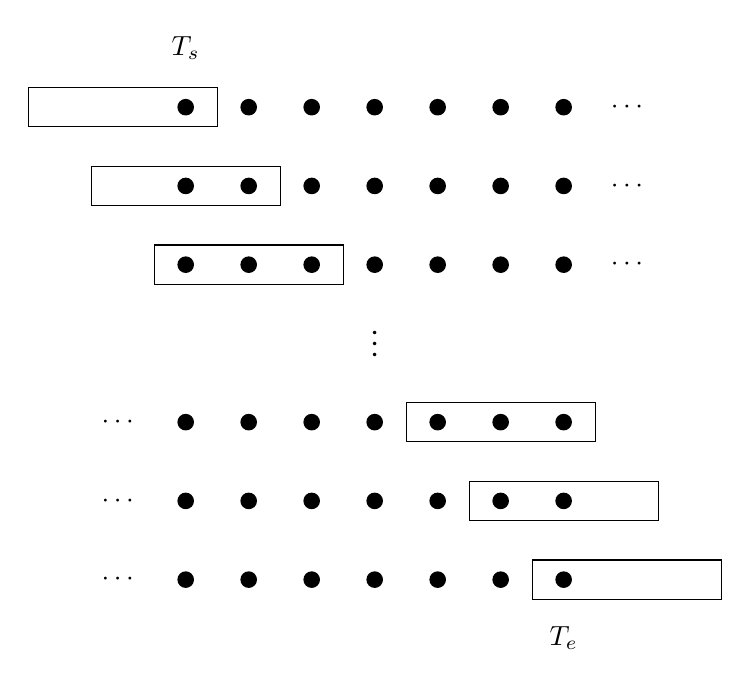
\begin{tikzpicture}

\def\interdotdistance{0.8}
\def\slidingwindowheight{0.5}

\newcommand\slidingwindowthingy[3]
{
    \foreach \i [evaluate=\i as \x using \i * \interdotdistance] in {0,...,6}
    {
        \fill (\x,#1) circle [color=black,radius=3pt] node (n#1\i) {};
    }
    \draw ({(-0.5+#2)*\interdotdistance},#1-0.5*\slidingwindowheight) rectangle +(3*\interdotdistance,\slidingwindowheight);
    \ifcase #3
        \node [right=10pt of n#16] {$ \cdots $};
    \or
        \node [left=10pt of n#10] {$ \cdots $};
    \fi
}

\slidingwindowthingy{0}{-2}{0}
\slidingwindowthingy{-1}{-1}{0}
\slidingwindowthingy{-2}{0}{0}

\node at (2.4,-2.9) {$ \vdots $};

\slidingwindowthingy{-4}{4}{1}
\slidingwindowthingy{-5}{5}{1}
\slidingwindowthingy{-6}{6}{1}

\node [above=10pt of n00] {$ T_s $};
\node [below=10pt of n-66] {$ T_e $};

\end{tikzpicture}
\caption{Visualization of the way algorithm~\ref{alg:rec-par-fwi} and further algorithms pass a sliding window over the sequence. Black dots represent timestamps that belong to the sequence, regardless of whether events occur at that timestamp.}
\label{fig:sliding-window}
\end{figure}

Recognition is accomplished as follows. For each event type $ A $, a counter $ A \text{.count} $ is maintained. This counter denotes how many events of type $ A $ are currently in the window. When a new event of type $ A $ enters the window (line~\ref{alglin:rec-par-fwi:new-events} and further), this counter is increased by $ 1 $. Then, for all episodes $ \alpha $ containing $ A \text{.count} $ nodes of type $ A $, a per-episode counter $ \alpha \text{.event\_count} $ is increased by $ A \text{.count} $, indicating that there are currently enough events of type $ A $ in the window to satisfy an occurrence. If this is the case for all event types in $ \alpha $, then $ \alpha \text{.event\_count} = | \alpha | $, and so the window contains $ \alpha $. To mark the point in time at which the episode entered the sliding window, variable $ \alpha \text{.in\_window} $ gets set to \emph{start}.

When an event of type $ A $ leaves the window (line~\ref{alglin:rec-par-fwi:old-events} and further), for all episodes $ \alpha $ with $ A \text{.count} $ nodes of event type $ A $, if $ \alpha \text{.event\_count} = | \alpha | $, $ \alpha $ has been contained in a number of windows, but is now no longer. The episode was in $ (\text{start} - \alpha \text{.in\_window}) $ windows, and so $ \alpha \text{.freq\_count} $ gets updated accordingly. Next, $ A \text{.count} $ gets decreased by $ 1 $ to reflect the fact that an event of type $ A $ has left the sliding window.

Figure~\ref{fig:parallel-recognition} illustrates this.

\begin{figure}
\centering

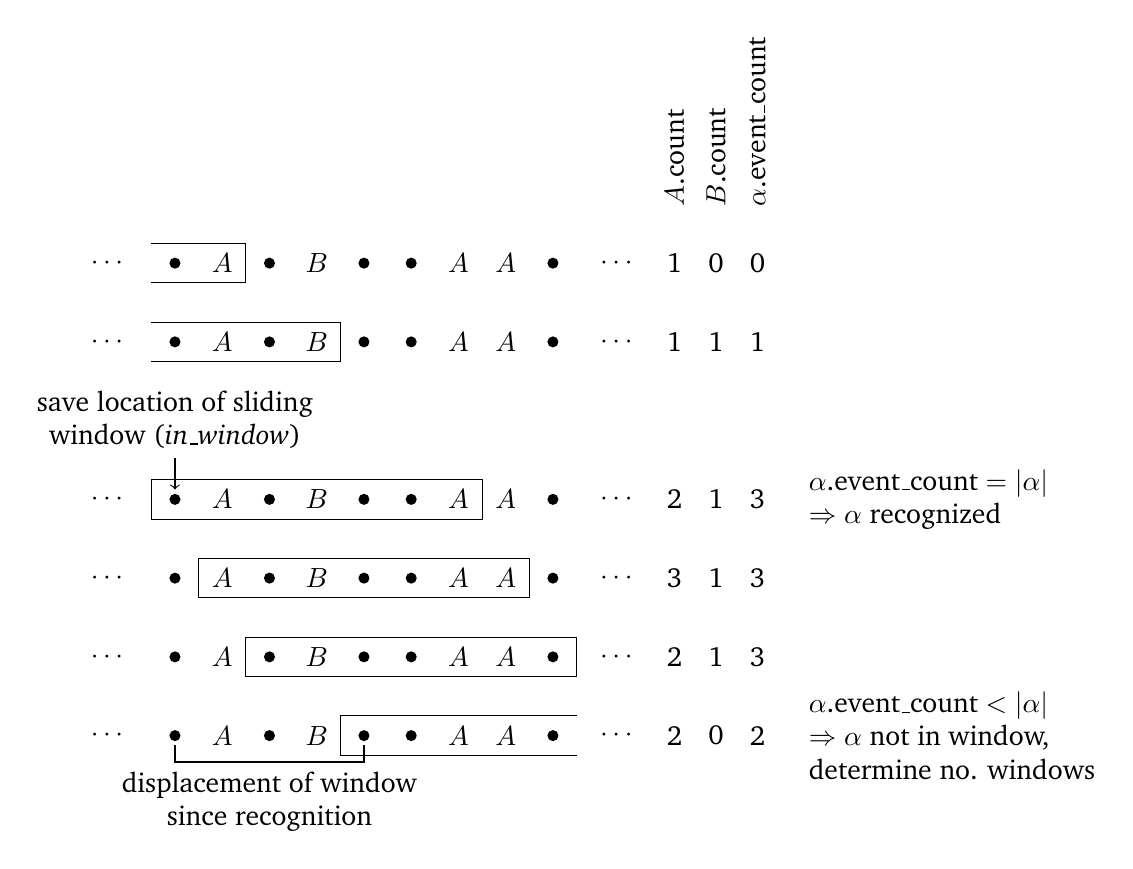
\begin{tikzpicture}


\def\slidingwindowheight{0.5}
\def\interdotdistance{0.6}

\newcommand\letteratposition[1]
{\ifnum#1=1A\else\ifnum#1=3B\else\ifnum#1=6A\else\ifnum#1=7A\else0\fi\fi\fi\fi}

\newcommand\slidingwindowthingy[2]
{
    \foreach \i [evaluate=\i as \x using \i * \interdotdistance] in {0,...,8}
    {
        \ifnum\pdfstrcmp{\letteratposition{\i}}{0}=0
            \fill (\x,#1) circle [color=black,radius=2pt] node (n#2-\i) {};
        \else
            \draw (\x,#1) node (n#2-\i) {$ \letteratposition{\i} $};
        \fi
    }

    \node (dr#2) [right=10pt of n#2-8] {$ \cdots $};
    \node (dl#2) [left=10pt of n#2-0] {$ \cdots $};
}

\slidingwindowthingy{0}{0}
\draw (-0.5*\interdotdistance,-0.5*\slidingwindowheight) -- ++(2*\interdotdistance,0) -- ++(0,\slidingwindowheight) -- ++(-2*\interdotdistance,0);
\node (Acount) [right=1em of dr0,rotate=90,anchor=west,xshift=0.6cm] {$ A \text{.count} $};
\node (Bcount) [right=2.5em of dr0,rotate=90,anchor=west,xshift=0.6cm] {$ B \text{.count} $};
\node (alphaeventcount) [right=4em of dr0,rotate=90,anchor=west,xshift=0.6cm] {$ \alpha \text{.event\_count} $};

\node at (Acount |- dr0) {1};
\node at (Bcount |- dr0) {0};
\node at (alphaeventcount |- dr0) {0};

\slidingwindowthingy{-1}{1}
\draw (-0.5*\interdotdistance,-1-0.5*\slidingwindowheight) -- ++(4*\interdotdistance,0) -- ++(0,\slidingwindowheight) -- ++(-4*\interdotdistance,0);
\node at (Acount |- dr1) {1};
\node at (Bcount |- dr1) {1};
\node at (alphaeventcount |- dr1) {1};

\slidingwindowthingy{-3}{2}
\draw (-0.5*\interdotdistance,-3-0.5*\slidingwindowheight) rectangle ++(7*\interdotdistance,\slidingwindowheight);
\node at (Acount |- dr2) {2};
\node at (Bcount |- dr2) {1};
\node at (alphaeventcount |- dr2) {3};
\node [right=5.5em of dr2,align=left] {$ \alpha \text{.event\_count} = | \alpha | $\\$ \Rightarrow \alpha $ recognized};
\node (inwindowtxt) [above=0.4cm of n2-0,align=center] {save location of sliding\\window (\emph{in\_window})};
\draw [->] (inwindowtxt) -- (n2-0);

\slidingwindowthingy{-4}{3}
\draw (0.5*\interdotdistance,-4-0.5*\slidingwindowheight) rectangle ++(7*\interdotdistance,\slidingwindowheight);
\node at (Acount |- dr3) {3};
\node at (Bcount |- dr3) {1};
\node at (alphaeventcount |- dr3) {3};

\slidingwindowthingy{-5}{4}
\draw (1.5*\interdotdistance,-5-0.5*\slidingwindowheight) rectangle ++(7*\interdotdistance,\slidingwindowheight);
\node at (Acount |- dr4) {2};
\node at (Bcount |- dr4) {1};
\node at (alphaeventcount |- dr4) {3};

\slidingwindowthingy{-6}{5};
\draw (8.5*\interdotdistance,-6-0.5*\slidingwindowheight) -- ++(-5*\interdotdistance,0) -- ++(0,\slidingwindowheight) -- ++(5*\interdotdistance,0);
\node at (Acount |- dr5) {2};
\node at (Bcount |- dr5) {0};
\node at (alphaeventcount |- dr5) {2};
\node [right=5.5em of dr5,align=left] {$ \alpha \text{.event\_count} < | \alpha | $\\$ \Rightarrow \alpha $ not in window,\\determine no. windows};

\draw (n5-0.south) -- ++(0,-6pt) -- node (numwindowsindicator) [midway,below,align=center] {displacement of window\\since recognition} ++(4*\interdotdistance,0) -- ++(n5-4);

\end{tikzpicture}

\caption{Recognition of parallel episode $ \alpha = \{ A, A, B \} $ using the fixed window frequency measure. Black dots are timestamps which don't contain $ A $ or $ B $.}
\label{fig:parallel-recognition}
\end{figure}

\subsection{Recognizing serial episodes with fixed windows}

\begin{algorithm}

\caption{Recognizing serial episodes using the fixed window frequency measure. \\
Input: An array of serial episodes $ \mathcal{C} $, an event sequence $ \boldsymbol{s} = (s, T_s, T_e) $, a window width \textit{win}, and a frequency threshold \textit{min\_fr}. \\
Ouptut: The episodes of $ \mathcal{C} $ that are frequent in $ \boldsymbol{s} $ with respect to \textit{win} and \textit{min\_fr}.
}

\begin{algorithmic}[1]

\LineComment{Initialization}
\ForAll{$ \alpha \in \mathcal{C} $}
    \For{$ i \leftarrow 1 $ to $ | \alpha | $}
        \State{$ \alpha \text{.initialized} \leftarrow \text{\textit{uninitialized}} $}
        \State{$ \text{waits}(\alpha[i]) \leftarrow \emptyset $}
    \EndFor
\EndFor

\ForAll{$ \alpha \in \mathcal{C} $}
    \State{$ \text{waits}(\alpha[1]) \leftarrow \text{waits}(\alpha[1]) \cup \left\{ \left( \alpha, 1 \right) \right\} $} \label{alglin:rec-ser-fwi:fill-waits-init}
    \State{$ \alpha \text{.freq\_count} \leftarrow 0 $}
\EndFor

\For{$ t \leftarrow T_s - \text{win} $ to $ T_s - 1 $} $ \text{begins\_at}(t) \leftarrow \emptyset $
\EndFor

\LineComment{Recognition}
\For{$ \text{start} \leftarrow T_s - \text{win} + 1 $ to $ T_e $} \label{alglin:rec-ser-fwi:iterate-sequence}
    \State{$ \text{begins\_at}(\text{start} + \text{win} - 1) \leftarrow \emptyset $}
    \State{$ \text{transitions} \leftarrow \emptyset $}
    \ForAll{events $ (A, t) $ in $ s $ such that $ t = \text{start} + \text{win} - 1 $} \label{alglin:rec-ser-fwi:iterate-new-events}
        \ForAll{$ ( \alpha, j) \in \text{waits}(A) $}
            \If{$ j = | \alpha | \wedge \alpha \text{.initialized}[j] = \text{\textit{uninitialized}} $} \label{alglin:rec-ser-fwi:mark-enter}
                \State{$ \alpha \text{.in\_window} \leftarrow \text{start} $}
            \EndIf
            \If{$ j = 1 $} \label{alglin:rec-ser-fwi:add-to-transitions}
                \State{$ \text{transitions} \leftarrow \text{transitions} \cup \{ ( \alpha, 1, \text{start} + \text{win} - 1 ) \} $}
            \Else
                \State{$ \text{transitions} \leftarrow \text{transitions} \cup \{ \alpha, j, \alpha \text{.initialized} [j - 1] \} $}
                \State{$ \text{begins\_at}( \alpha \text{.initialized}[j - 1] ) \leftarrow $ \label{alglin:rec-ser-fwi:cleanup-old-states}
                \State \hspace{\algorithmicindent} $ \text{begins\_at}( \alpha \text{.initialized}[j - 1] ) \setminus \{ ( \alpha, j - 1 ) \} $}
                \State{$ \alpha \text{.initialized} [j - 1] \leftarrow \text{\textit{uninitialized}} $}
                \State{$ \text{waits}(A) \leftarrow \text{waits}(A) \setminus \{ ( \alpha, j ) \} $}
            \EndIf
        \EndFor
    \EndFor
    \ForAll{$ ( \alpha, j, t ) \in \text{transitions} $}
        \State{$ \alpha \text{.initialized} [j] \leftarrow t $} \label{alglin:rec-ser-fwi:transition-begin}
        \State{$ \text{begins\_at}(t) \leftarrow \text{begins\_at}(t) \cup \{ ( \alpha, j ) \} $}
        \If{$ j < | \alpha | $}
            \State{$ \text{waits}(\alpha [j + 1]) \leftarrow \text{waits}(\alpha [j + 1]) \cup \{ (\alpha, j + 1) \} $} \label{alglin:rec-ser-fwi:transition-end}
        \EndIf
    \EndFor
    \ForAll{$ (\alpha, l) \in \text{begins\_at}(\text{start} - 1) $} \label{alglin:rec-ser-fwi:cleanup-for}
        \If{$ l = | \alpha | $} \label{alglin:rec-ser-fwi:cleanup-iteration-begin}
            \State{$ \alpha \text{.freq\_count} \leftarrow \alpha \text{.freq\_count} - \alpha \text{.in\_window} + \text{start} $}
        \Else
            \State{$ \text{waits}(\alpha [l + 1]) \leftarrow \text{waits}(\alpha [l + 1]) \setminus \{ ( \alpha, l + 1 ) \} $}
        \EndIf
        \State{$ \alpha \text{.initialized}[l] \leftarrow \text{\textit{uninitialized}} $} \label{alglin:rec-ser-fwi:cleanup-iteration-end}
    \EndFor
\EndFor
\ForAll{episodes $ \alpha $ in $ \mathcal{C} $}
    \If{$ \alpha \text{.freq\_count} / (T_e - T_s + \text{win} - 1) \geq \text{min\_fr} $}
        \State{output $ \alpha $}
    \EndIf
\EndFor

\end{algorithmic}

\label{alg:rec-ser-fwi}
\end{algorithm}

Algorithm~\ref{alg:rec-ser-fwi} is for recognizing serial episodes in a sequence. By definition serial episodes impose a total order on the nodes, and consequently on the events in the sequence in order to satisfy an occurrence of an episode. Serial episodes are therefore recognized using simple automata, instances of which advance state as events are encountered. Just like the algorithm for recognizing parallel episodes, algorithm~\ref{alg:rec-ser-fwi} iterates over the sequence once.

Each episode has its own automaton, which consists of $ | \alpha | $ states: each state corresponds to a node in the episode. For an episode $ A_1 \to A_2 \to \cdots A_n $, state $ j $ refers to the node with event type $ A_j $. Then an instance of the automaton for $ \alpha $ being in a state $ j $ denotes that the episode has been recognized up to (and including) the $ j $-th node. When in state $ j $ and upon encountering an event of which the type corresponds to the type of the $ (j + 1) $-th node of the episode, the instance will transition to state $ j + 1 $.

When an automaton instance of $ \alpha $ reaches state $ | \alpha | $, the episode has been successfully recognized, and from that point on, the episode will occur in a number of windows as the sliding window slides over the sequence.

Regardless of the state an automaton instance reached, the instance is removed when the timestamp at which the instance was initialized falls out of the sliding window.

Figure~\ref{fig:serial-recognition} illustrates the principle with an example.

\begin{figure}
\centering

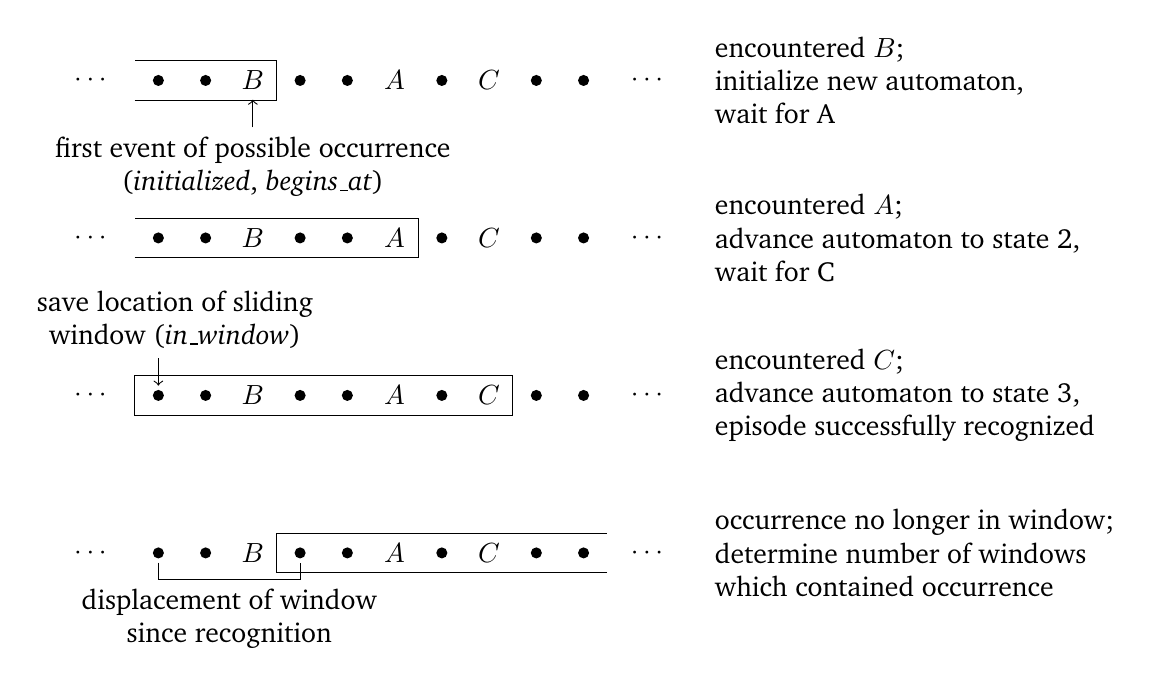
\begin{tikzpicture}

\def\slidingwindowheight{0.5}
\def\interdotdistance{0.6}

\newcommand\letteratposition[1]
{\ifnum#1=2B\else\ifnum#1=5A\else\ifnum#1=7C\else0\fi\fi\fi}

\newcommand\slidingwindowthingy[2]
{
    \foreach \i [evaluate=\i as \x using \i * \interdotdistance] in {0,...,9}
    {
        \ifnum\pdfstrcmp{\letteratposition{\i}}{0}=0
            \fill (\x,#1) circle [color=black,radius=2pt] node (n#2-\i) {};
        \else
            \draw (\x,#1) node (n#2-\i) {$ \letteratposition{\i} $};
        \fi
    }

    \node (dr#2) [right=10pt of n#2-9] {$ \cdots $};
    \node (dl#2) [left=10pt of n#2-0] {$ \cdots $};
}

\slidingwindowthingy{0}{0}
\draw (-0.5*\interdotdistance,-0.5*\slidingwindowheight) -- ++(3*\interdotdistance,0) -- ++(0,\slidingwindowheight) -- ++(-3*\interdotdistance,0);
\node [right=10pt of dr0,align=left] {encountered $ B $;\\initialize new automaton,\\wait for A};
\node (initializedtxt) [below=0.35cm of n0-2,align=center] {first event of possible occurrence\\(\emph{initialized}, \emph{begins\_at})};
\draw [->] (initializedtxt) -- (n0-2);

\slidingwindowthingy{-2}{1}
\draw (-0.5*\interdotdistance,-2-0.5*\slidingwindowheight) -- ++(6*\interdotdistance,0) -- ++(0,\slidingwindowheight) -- ++(-6*\interdotdistance,0);
\node [right=10pt of dr1,align=left] {encountered $ A $;\\advance automaton to state 2,\\wait for C};

\slidingwindowthingy{-4}{2}
\draw (-0.5*\interdotdistance,-4-0.5*\slidingwindowheight) rectangle ++(8*\interdotdistance,\slidingwindowheight);
\node [right=10pt of dr2,align=left] {encountered $ C $;\\advance automaton to state 3,\\episode successfully recognized};
\node (marktxt) [above=0.35cm of n2-0,align=center,xshift=6pt] {save location of sliding\\window (\emph{in\_window})};
\draw [->] (n2-0 |- marktxt.south) -- (n2-0);

\slidingwindowthingy{-6}{3}
\draw ({(9.5)*\interdotdistance},-6-0.5*\slidingwindowheight) -- ++(-7*\interdotdistance,0) -- ++(0,\slidingwindowheight) -- ++(7*\interdotdistance,0);
\node [right=10pt of dr3,align=left] {occurrence no longer in window;\\determine number of windows\\which contained occurrence};

\draw (n3-0.south) -- ++(0,-6pt) -- node (numwindowsindicator) [midway,below,align=center] {displacement of window\\since recognition} ++(3*\interdotdistance,0) -- (n3-3.south);

\end{tikzpicture}

\caption{Illustration for the recognition of serial episode $ B \to A \to C $. Black dots are timestamps which don't contain $ B $, $ A $ or $ C$.}
\label{fig:serial-recognition}
\end{figure}

\subsubsection{Data structures}

The algorithm uses some bookkeeping data structures, which get updated as the sequence gets read. We'll discuss the most important ones.
\begin{itemize}
\item \textbf{waits} maps an event type to a set of pairs of the form $ (\alpha, j) $, where $ \alpha $ is an episode and $ j $ represents a state in the episode's automaton. If a pair $ (\alpha, j) $ is in $ \text{waits}(A) $, and $ j > 1 $, then $ \alpha $ has an instance of its automaton currently in state $ (j - 1) $ and is waiting for an event of type $ A $ to advance to the next state. Throughout the iteration over the sequence, $ \text{waits}(\alpha[1]) $ will always contain $ (\alpha, 1) $ for each episode $ \alpha $, since a new automaton instance should be instantiated any time the first event of a serial episode occurs.
\item \textbf{begins\_at} maps a timestamp to a set of pairs $ (\alpha, j) $. If $ (\alpha, j) $ is in $ \text{begins\_at}(t) $, then $ \alpha $ has an instance of its automaton in state $ j $, and it was initialized at timestamp $ t $.
\item Each episode $ \alpha $ has an $ | \alpha | $-element array called \textbf{initialized}, where $ \alpha \text{.initialized}[j] $ contains the timestamp in the sequence at which the instance currently in state $ j $ was initialized. If for a certain state there is currently no active instance, its corresponding element in the initialized array will be some special value---\cite{winepi97} chose 0, which we changed to \emph{uninitialized} for clarity and such that 0 can be a valid timestamp if necessary.

Note that \emph{initialized} allows at most one automaton to be in a given state at any time. This approach works because it is not useful to have multiple instances in the same state. If one automaton instance reaches a common state with another instance, they will simply make transitions simultaneously until the earlier instance gets removed. It suffices to maintain the instance which was reached the common state last, since it was initialized at a later timestamp, and thus will be the last to be removed.
\item All of the state transitions to be performed for a given timestamp are collected in a list, \textbf{transitions}, before they actually get executed. If they were executed immediately, an automaton could be incorrectly overwritten if there there are multiple events in a single timestamp. We will come back to this later.
\end{itemize}

\subsubsection{Operation}

With the data structures just described in mind, we will go through the algorithm in detail to see how it operates.

The initialization is rather straightforward. One thing to note is that the permanent pairs of the \emph{waits} sets are constructed (line~\ref{alglin:rec-ser-fwi:fill-waits-init}). As stated before, for each episode $ \alpha $, $ \text{waits}(\alpha[1]) $ contains $ (\alpha, 1) $ from the start, and throughout the algorithm, to initialize a new automaton instance for $ \alpha $ any time an event of type $ \alpha[1] $ occurs.

Then a sliding window is passed over the sequence, in the same manner algorithm~\ref{alg:rec-par-fwi} does (line~\ref{alglin:rec-ser-fwi:iterate-sequence}). Each time the sliding window is advanced, first the events that just came into the window are processed (line~\ref{alglin:rec-ser-fwi:iterate-new-events}), at time $ (\text{start} + \text{win} - 1) $. Say an event of type $ A $ came in. Thanks to the \emph{waits} data structure, all automaton instances that should make a state transition are found efficiently. For each of the pairs $ (\alpha, j) $ in $ \text{waits}(A) $, the following steps are evaluated:

\begin{enumerate}
\item (Lines~\ref{alglin:rec-ser-fwi:mark-enter} and further) If the automaton instance has reached state $ | \alpha | $, that is, the episode now occurs within the sliding window\footnote{This is not entirely correct. Note that new events coming into the window are processed before old events are removed. After processing new events, the oldest possible automata were therefore initialized at timestamp $ \text{start} - 1 $, which may cause an episode to be recognized without being in the current window $ s[\text{start}, \text{start} + \text{win}] $. However, for such a falsely recognized episode, the corresponding automaton will be removed immediately afterwards, and the displacement of the sliding window will be zero, thus not affecting $ \alpha $'s frequency count.}, then $ \alpha \text{.in\_window} $ gets set to \emph{start} to mark the time at which the episode entered the sliding window. Except if another instance is already in state $ | \alpha | $, then $ \alpha \text{.in\_window} $ was already set. If we would overwrite the value in that case, the windows covering the previous occurrence would not be counted.
\item (Lines~\ref{alglin:rec-ser-fwi:add-to-transitions} and further) The transition to be made is captured in the list of transitions.
\item (Lines~\ref{alglin:rec-ser-fwi:cleanup-old-states} and further) The old state information is removed from data structures \emph{begins\_at}, \emph{initialized}, and \emph{waits}, if we're not initializing a new automaton instance.
\end{enumerate}

When all new events have been processed, the transitions are finalized: the new state information is written to \emph{initialized}, \emph{begins\_at}, and \emph{waits}.

After applying the state transitions, the events no longer in the window are dropped. This entails looking up all automata which were instantiated at timestamp $ (\text{start} - 1) $ using the \emph{begins\_at} data structure (line~\ref{alglin:rec-ser-fwi:cleanup-iteration-begin} and further):

\begin{enumerate}
\item If the automaton instance was in state $ | \alpha | $, the episode occurred within the window until now. When the episode was first recognized to occur in the sliding window, the location of the sliding window was stored in $ \alpha \text{.in\_window} $, and so the number of fixed windows in which the episode occurred can be determined by the displacement of the sliding window since then.
\item If the automaton instance was not in state $ | \alpha | $, the \emph{waits} data structure is updated to reflect the removal of the instance.
\item The \emph{initialized} array of the episode is updated to reflect the removal of the automaton instance.
\end{enumerate}

\subsubsection{Correcting the original algorithm pseudocode}

While implementing this algorithm we found an oversight in~\cite{winepi97} for the pseudocode of algorithm~\ref{alg:rec-ser-fwi} (algorithm~5 in~\cite{winepi97}), related to multiple instances of an episode's automaton reaching a common state. At line~\ref{alglin:rec-ser-fwi:transition-begin}, a transition of an automaton instance is being applied. The \emph{initialized} array gets updated, potentially overwriting a previous instance in the same state. \emph{begins\_at} gets updated with the new state, but the information about the potentially overwritten instance is not removed from \emph{begins\_at}. We'll illustrate how this affects the output with an example.

Using a window width of 2, and scanning the subsequence $ \cdots E \: A \: E \: C \cdots $. Say that the first $ E $ has timestamp $ t_1 $. Consider the recognition of the serial episode $ \alpha = E \to C $. Obviously the subsequence contains $ \alpha $, and a window width of 2 suffices to recognize an instance of the episode in the subsequence. Upon encountering the first $ E $, an automaton instance gets initialized for $ \alpha $ (lines \ref{alglin:rec-ser-fwi:transition-begin} through \ref{alglin:rec-ser-fwi:transition-end}). This includes, as discussed before:
\begin{itemize}
\item setting the timestamp in the \emph{initialized} array;
\item adding $ (\alpha, 2) $ to the $ \text{waits}(C) $ set (so that if $ C $ is encountered, the automaton can transition to the next state);
\item adding $ (\alpha, 1) $ to $ \text{begins\_at}(t_1) $ (to facilitate the removal of the the automaton instance once $ t_1 $ falls out of the window).
\end{itemize}

When the second $ E $ is read (at $ t = t_1 + 2 $ and when $ \text{start} = t_1 + 1 $), a new instance of the automaton is created, and since the previous instance is still in state $ 1 $---no $ C $ has been encountered---the previous instance must be overwritten. Indeed, this happens for the \emph{initialized} data structure at line~\ref{alglin:rec-ser-fwi:transition-begin}. However, \emph{begins\_at} is never updated to reflect this: $ (\alpha, 1) $ remains in $ \text{begins\_at}(t_1) $. Because of this, the newly created automaton is wrongly removed just afterwards, because the first instance fell out of the window (while iterating $ \text{begins\_at}(t_1 = \text{start} - 1) $, line~\ref{alglin:rec-ser-fwi:cleanup-for}). Then $ (\alpha, 2) $ is no longer in $ \text{waits}(C) $, and $ \alpha $ will fail to be recognized.

This is a problem any time an older instance of an episode's automaton instance gets overwritten by a more recent one reaching the same state. In some cases, as illustrated above, an occurrence of an episode may fail to be recognized entirely, while in other cases it may get recognized but with an incorrect frequency count, again due to an automaton instance being removed early. Consequently, this may cause the episode to be considered infrequent while it actually is frequent.

\subsubsection{The necessity of the \emph{transitions} data structure}

Earlier we mentioned that the \emph{transitions} data structure, which captures all transitions to execute at a timestamp before finalizing them, exists for good reason. In short, an automaton instance in state $ j $ could incorrectly overwrite an instance in state $ j + 1 $ if both instances are to transition. Consider the following example. Say $ \alpha = A \to B \to C $ is in the collection of candidates, and consider the event sequence $ \langle (A, 1),\allowbreak(B, 2),\allowbreak(A, 3),\allowbreak(B, 4),\allowbreak(C, 4) \rangle $. Note that the last two events occur at the same timestamp. Assume the window width is at least 4 so that it is sufficiently large to recognize $ \alpha $.

\begin{enumerate}
\item When $ (A, 1) $ enters the window, a new automaton for $ \alpha $ gets initialized.
\item When $ (B, 2) $ comes in, the automaton transitions to state~$ 2 $.
\item When $ (A, 3) $ comes in, a new automaton instance for $ \alpha $ is initialized. Now $ \alpha $'s \emph{initialized} array contains:
\begin{align*}
\langle 1, 3, \text{\textit{uninitialized}} \rangle
\end{align*}
\item Next, $ (B, 4) $ comes in. The most recently initialized instance will transition to state $ 2 $. \label{B4-comes-in}
\item Finally, $ (C, 4) $ enters the window. The oldest automaton instance should transition to state $ 3 $.
\end{enumerate}

Now, if at step~\ref{B4-comes-in} the transition was performed immediately, then the \emph{initialized} entry of the older automaton instance would have be incorrectly overwritten:
\begin{align*}
\langle \text{\textit{uninitialized}}, 1, \text{\textit{uninitialized}} \rangle
\end{align*}
Now the data structures are in an inconsistent state.

Collecting all transitions to be peformed at a given timestamp before executing them, will prevent \emph{initialized} entries being incorrectly overwritten.

\subsection{Recognizing parallel episodes with minimal windows}

\begin{algorithm}

\caption{Recognizing a collection $ \mathcal{C} $ of parallel episodes in a sequence $ s $ using the minimal window frequency measure. \\
Input: A collection $ \mathcal{C} $ of parallel episodes, an event sequence $ \boldsymbol{s} = (s, T_s, T_e) $, a window width \textit{win}, and a frequency threshold \textit{min\_fr}. \\
Output: The episodes of $ \mathcal{C} $ that are frequent in $ \boldsymbol{s} $ with respect to \textit{win} and \textit{min\_fr}.}

\begin{algorithmic}[1]

\LineComment{Initialization}
\ForAll{event types $ A $}
    \State $ \text{in\_window}(A) \gets \text{empty queue} $
\EndFor
\ForAll{$ \alpha $ in $ \mathcal{C} $}
    \ForAll{$ A $ in $ \alpha $}
        \State $ \text{consider\_max}(\alpha, A) \gets 0 $
        \State $ \text{num\_needed}(\alpha, A) \gets \text{number of elements of type $ A $ in $ \alpha $} $
        \State $ \text{contains}(A) \gets \text{contains}(A) \cup \{ \alpha \} $
    \EndFor
\EndFor

\LineComment{Recognition}
\For{$ \text{start} \gets T_s - \text{win} + 1 $ to $ T_e - 1 $} % TODO check if starting at correct position
    \LineComment{Drop out old events from the window}
    \ForAll{events $ (A, t) $ in $ s $ such that $ t = \text{start} - 1 $}
        \While{$ | \text{in\_window}(A) | > 0 \wedge \text{in\_window}(A) \text{.front}() < \text{start} $}
            \State $ \text{in\_window}(A) \text{.pop}() $
        \EndWhile
    \EndFor

    \LineComment{Bring in new events to the window}
    \ForAll{events $ (A, t) $ in $ s $ such that $ t = \text{start} + \text{win} - 1 $}
        \State $ \text{in\_window}[A] \text{.push}(t + \text{win} - 1) $
        \ForAll{$ \alpha $ in $ \text{contains}(A) $}
            \If{{\footnotesize $ \forall A $ in $ \alpha : \min(| \text{in\_window}(A) |, \text{consider\_max}(\alpha, A)) \geq \text{num\_needed}(\alpha, A) $ }}
                \LineComment{Occurrence detected; determine start of minimal window}
                \State $ Q \gets \text{in\_window}(A) $
                \State $ \text{window\_start} \gets \min\{ t | \forall A $ in $ \alpha : t = Q[| Q | - \text{num\_needed}(\alpha, A) + 1] \} $
                \ForAll{$ A $ in $ \alpha $}
                    $ Q \gets \text{in\_window}(A) $
                    \If{$ \text{window\_start} = Q[| Q | - \text{num\_needed}(\alpha, A)) + 1] $}
                        \State $ \text{consider\_max}(\alpha, A) \gets \text{num\_needed}(\alpha, A) - 1 $
                    \EndIf
                    \State append $ [\text{window\_start}, \text{start} + \text{win}) $ to $ \alpha \text{.minimal\_windows} $
                \EndFor
            \EndIf
        \EndFor
    \EndFor
\EndFor

\end{algorithmic}

\label{alg:rec-par-mwi}
\end{algorithm}

With minimal windows, the frequency of an episode isn't expressed in terms of a number of windows anymore, but in the number of actual occurrences of the episode. For the fixed window frequency measure, % TODO finish sentence (and by extension, thesis)

\subsection{Recognizing serial episodes with minimal windows}

\begin{algorithm}

\caption{Recognizing serial episodes using the minimal window frequency measure. \\
Input: An array of serial episodes $ \mathcal{C} $, an event sequence $ \boldsymbol{s} = (s, T_s, T_e) $, a window width \textit{win}, and a frequency threshold \textit{min\_fr}. \\
Ouptut: The episodes of $ \mathcal{C} $ that are frequent in $ \boldsymbol{s} $ with respect to \textit{win} and \textit{min\_fr}.
}

\begin{algorithmic}[1]

\LineComment{Initialization}
\ForAll{$ \alpha \in \mathcal{C} $}
    \For{$ i \leftarrow 1 $ to $ | \alpha | $}
        \State{$ \alpha \text{.initialized}[i] \leftarrow \text{\textit{uninitialized}} $}
        \State{$ \text{waits}(\alpha[i]) \leftarrow \emptyset $}
    \EndFor
\EndFor

\ForAll{$ \alpha \in \mathcal{C} $}
    \State{$ \text{waits}(\alpha[1]) \leftarrow \text{waits}(\alpha[1]) \cup \left\{ \left( \alpha, 1 \right) \right\} $} \label{alglin:rec-ser-mwi:fill-waits-init}
    \State{$ \alpha \text{.minimal\_windows} \gets \emptyset $}
\EndFor

\For{$ t \leftarrow T_s - \text{win} $ to $ T_s - 1 $} $ \text{begins\_at}(t) \leftarrow \emptyset $
\EndFor

\LineComment{Recognition}
\For{$ \text{start} \leftarrow T_s - \text{win} + 1 $ to $ T_e $} \label{alglin:rec-ser-mwi:iterate-sequence}
    \State{$ \text{begins\_at}(\text{start} + \text{win} - 1) \leftarrow \emptyset $}
    \State{$ \text{transitions} \leftarrow \emptyset $}
    \ForAll{$ (\alpha, l) \in \text{begins\_at}(\text{start} - 1) $} \label{alglin:rec-ser-mwi:cleanup-for}
        \If{$ l < | \alpha | $} \label{alglin:rec-ser-mwi:cleanup-iteration-begin}
            \State{$ \text{waits}(\alpha [l + 1]) \leftarrow \text{waits}(\alpha [l + 1]) \setminus \{ ( \alpha, l + 1 ) \} $}
        \EndIf
        \State{$ \alpha \text{.initialized}[l] \leftarrow \text{\textit{uninitialized}} $} \label{alglin:rec-ser-mwi:cleanup-iteration-end}
    \EndFor
    \ForAll{events $ (A, t) $ in $ s $ such that $ t = \text{start} + \text{win} - 1 $} \label{alglin:rec-ser-mwi:iterate-new-events}
        \ForAll{$ ( \alpha, j) \in \text{waits}(A) $}
            \If{$ j = 1 $} \label{alglin:rec-ser-mwi:add-to-transitions}
                \State{$ \text{transitions} \leftarrow \text{transitions} \cup \{ ( \alpha, 1, \text{start} + \text{win} - 1 ) \} $}
            \Else
                \State{$ \text{transitions} \leftarrow \text{transitions} \cup \{ \alpha, j, \alpha \text{.initialized} [j - 1] \} $}
                \State{$ \text{begins\_at}( \alpha \text{.initialized}[j - 1] ) \leftarrow $ \label{alglin:rec-ser-mwi:cleanup-old-states}
                \State \hspace{\algorithmicindent} $ \text{begins\_at}( \alpha \text{.initialized}[j - 1] ) \setminus \{ ( \alpha, j - 1 ) \} $}
                \State{$ \alpha \text{.initialized} [j - 1] \leftarrow \text{\textit{uninitialized}} $}
                \State{$ \text{waits}(A) \leftarrow \text{waits}(A) \setminus \{ ( \alpha, j ) \} $}
            \EndIf
        \EndFor
    \EndFor
    \ForAll{$ ( \alpha, j, t ) \in \text{transitions} $}
        \State{$ \alpha \text{.initialized} [j] \leftarrow t $} \label{alglin:rec-ser-mwi:transition-begin}
        \State{$ \text{begins\_at}(t) \leftarrow \text{begins\_at}(t) \cup \{ ( \alpha, j ) \} $}
        \If{$ j = | \alpha | $}
            \State $ \alpha \text{.minimal\_windows} \gets $
            \State \hspace{\algorithmicindent} $ \alpha \text{.minimal\_windows} \cup \{ [\alpha \text{.initialized}[j], \text{start} + \text{win}) \} $
        \Else
            \State{$ \text{waits}(\alpha [j + 1]) \leftarrow \text{waits}(\alpha [j + 1]) \cup \{ (\alpha, j + 1) \} $} \label{alglin:rec-ser-mwi:transition-end}
        \EndIf
    \EndFor
\EndFor

\ForAll{episodes $ \alpha $ in $ \mathcal{C} $}
    \LineComment{See algorithm~\ref{alg:disjoint-window-frequency} in section~\ref{sec:disjoint-window-frequency}}
    \If{$ fr_m(\alpha) \geq \text{min\_fr} $}
        \State{output $ \alpha $}
    \EndIf
\EndFor

\end{algorithmic}

\label{alg:rec-ser-mwi}
\end{algorithm}

While recognizing parallel episodes with minimal windows was slightly more complicated than with fixed windows, recognizing serial episodes with minimal windows is actuallly simpler than with fixed windows, and can be accomplished with small changes to algorithm~\ref{alg:rec-ser-fwi}.

\subsection{Determining the disjoint-window frequency for the minimal windows frequency measure}
\label{sec:disjoint-window-frequency}

The disjoint-window frequency of an episode $ \alpha $ was previously defined as
\begin{align*}
fr_m(\alpha) = \max \{ | W | \mid W \subseteq mw(\alpha), dis(W) = 1 \}
\end{align*}

\begin{algorithm}

\caption{Determining the disjoint-window frequency of an episode.\\
Input: List $ W $ of minimal windows of the episode in a sequence $ s $, ordered by time in the sequence.\\
Output: The episode's disjoint-window frequency in $ s $.
}

\begin{algorithmic}[1]

\State $ u \gets 0 $
\State $ b_l \gets -\infty $
\ForAll {$ [a, b) \in W $}
    \If {$ b_l \leq a $}
        \State $ u \gets u + 1 $
        \State $ b_l \gets b $
    \EndIf
\EndFor
\State output $ u $

\end{algorithmic}

\label{alg:disjoint-window-frequency}
\end{algorithm}

In words, the disjoint-window frequency of an episode is the largest possible number of non-overlapping minimal windows that cover the episode.

Given a list of all of the minimal windows that cover an episode, the disjoint window frequency can be calculated as follows. Count the first window, if the list is not empty. Then, while iterating the list, count a window if it does not overlap with the window that was counted last. % TODO continue writing this

\iffalse
\begin{figure}

\tikzset{counted/.style={green!80!black},
    skipped/.style={red,dashed}}

\begin{subfigure}[b]{\textwidth}
\centering

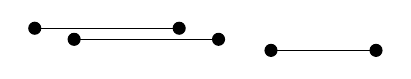
\begin{tikzpicture}

\draw [*-*] (0,0) -- (2,0);
\draw [*-*] (0.5,-4pt) -- (2.5,-4pt);
\draw [*-*] (3.0,-8pt) -- (4.5,-8pt);
% \draw (0,-2pt) rectangle (3,12pt);
% \draw (2.5,-4pt) rectangle (6,14pt);
% \draw (4,-2pt) rectangle (7,12pt);
% \draw (5,0pt) rectangle (10,10pt);

\end{tikzpicture}

\caption{A possible chain of overlapping minimal windows.}
\end{subfigure}
\par\bigskip
\begin{subfigure}[b]{\textwidth}
\centering

\begin{tikzpicture}

\draw [*-*,counted] (0,0) -- (3,0);
\draw [*-*,skipped] (2.5,-4pt) -- (6,-4pt);
\draw [*-*,counted] (4,-8pt) -- (7,-8pt);
\draw [*-*,skipped] (5,-12pt) -- (10,-12pt);

\end{tikzpicture}

\caption{Selecting the largest number of disjoint windows. Dashed line means not selected.}
\end{subfigure}
\par\bigskip
\begin{subfigure}[b]{\textwidth}
\centering

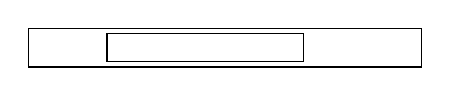
\begin{tikzpicture}

\draw (0,-2pt) rectangle (5,12pt);
\draw (1,0pt) rectangle (3.5,10pt);

\end{tikzpicture}

\caption{An impossible set of minimal windows: one window cannot be contained in another.}
\end{subfigure}

\caption{Visualizing the minimal windows of an episode.}
\label{fig:minimal-windows-chains}
\end{figure}
\fi

\subsection{Removing episodes which have been found infrequent}
\label{sec:maintain-blocks}

\begin{algorithm}

\caption{Removing infrequent episodes from a collection of candidates $ \mathcal{C} $ for which \emph{freq\_count} is known. \\
Input: A sorted array of candidates $ \mathcal{C} $, including their \emph{block\_start} values, and their \emph{freq\_count} values with respect to some sequence, and a minimum frequency threshold \emph{min\_fr}. \\
Output: A sorted array $ \mathcal{F} $ of those episodes in $ \mathcal{C} $ which are frequent, along with consistent \emph{block\_start} values.
}

\begin{algorithmic}[1]

\State $ \text{new\_block\_start} \gets 1 $
\State $ \mathcal{F} \gets \text{empty array} $
\State $ \mathcal{F} \text{.block\_start} \gets \text{empty array} $
\For{$ i = 1 $; $ i \leq | \mathcal{C} | $; $ i \gets i + 1 $}
    \If{$ \alpha \text{.freq\_count} < \text{min\_fr} $}
        \LineComment{Episode infrequent; discard}
        \State continue with next i
    \EndIf
    \If{$ \mathcal{C} \text{.block\_start}[i] = i $} \label{alglin:remove-infrequent-episodes:different-block-test}
        \LineComment{Encountered new block in candidates}
        \State $ \text{new\_block\_start} \gets | \mathcal{F} | $
    \EndIf
    \State append $ \alpha $ to $ \mathcal{F} $
    \State $ \mathcal{F} \text{.block\_start}[ | \mathcal{F} | ] \gets \text{new\_block\_start} $
\EndFor
\State output $ \mathcal{F} $

\end{algorithmic}

\label{alg:remove-infrequent-episodes}
\end{algorithm}

At first sight, it seems a trivial task to discard episodes from a list of candidates which have turned out to be infrequent. But one thing needs to be taken into consideration, namely the auxiliary \emph{block\_start} variables, used in the candidate generation algorithm (section~\ref{sec:cand-gen}). Each episode $ \alpha $ has such a \emph{block\_start} value, which denotes the array index of the first episode in the list for which it shares the first $ \alpha - 1 $ elements in the episode's array representation. If we remove episodes without further consideration, these indices will be invalidated. They should not be invalidated, however, since the next round of the candidate generation step relies on them. Hence we need to keep track of the blocks while constructing the list of frequent episodes. Algorithm~\ref{alg:remove-infrequent-episodes} achieves this.

The algorithm stores the frequent episodes in a new data structure $ \mathcal{F} $. While iterating over the episodes in order, the array index of the new block start is kept. If for an index $ i $, $ \mathcal{C}. \text{block\_start}[i] = i $, we know that a new block started at position $ i $ in $ \mathcal{C} $, and so \emph{new\_block\_start} gets updated in order to start a new block in $ \mathcal{F} $ as well.

\newpage


\chapter{Experiments}
\label{sec:experiments}

In this section, we perform experiments to answer the research question we posed in the introduction. Concisely put, we want to know whether we can find patterns in long sequences in a reasonable time, and whether there are interesting patterns to be found.

After choosing a number of datasets and showing some of their basic characteristics, we assess the performance of the implementation by running it on datasets of different kinds, and varying the parameter.

First, we'll briefly discuss how we ensured the correctness of our implementation.

\section{Correctness}

A big point of comparison while implementing our algorithms was a closed episode miner\footnote{http://adrem.ua.ac.be/mining-closed-strict-episodes}. It allowed us to verify the correctness of our implementation. The closed episode miner differs in a few ways from our implementation:

\begin{itemize}
\item It mines general episodes, not just parallel and serial episodes.
\item It mines closed episodes. An episode is closed if there are no superepisodes of the same frequency. Mining only closed episodes helps reduce the amount of output, by excluding non-closed episodes. The closed episode miner has options to mine non-closed episodes as well, which allows us to compare the output of both implementations.
\item While our implementation finds episodes of one class at a time, as specified by the user --- parallel or serial --- the closed episode miner finds episodes of all classes at once --- parallel, serial and general.
\end{itemize}

Given the above, in order to compare the two implementations in terms of their output, we have to enable the options that cause the closed episode miner to find non-closed episodes, since our implementation does not exclude non-closed episodes; and we have to filter out those episodes which don't match the class of episodes we're currently mining.

\iffalse
Mining general episodes is of higher complexity than parallel and serial episodes.

Parallel episodes can only ``grow'' by adding a new node, and serial episodes grow in much the same way: by adding a node and an edge at the same time. Pattern explosion is a bigger concern with general episodes: additionally, they can grow by adding only an edge. So, ideally, our implementation should be faster than the closed episode miner.

% TODO include this somehow?
\fi

We validated the output of our implementation with the output of the closed episode miner, running the closed episode miner alongside our implementation on the same datasets and parameter configurations, then parsing and comparing the results. Thanks to the closed episode miner we were able to eliminate quite a few errors in our implementation.

We did find, however, a possible bug in the closed episode miner. When mining parallel episodes in the example sequence (Figure~\ref{fig:event-sequence}), using the weighted-window frequency and with a window width of 8, the frequencies for a few episodes differed, as shown in table~\ref{table:closepi-frequency-difference}. Observing the sequence, each of these episodes has two overlapping minimal windows, of which the second one has a greater weight. Our implementation seems to correctly select the window with the higher weight, while the closed episode miner seems to choose the first window.

Further distilling the issue, we tested a simpler example: the sequence $ \langle (a, 1),\allowbreak(a, 3),\allowbreak(a, 4) \rangle $, episode $ \{ a, a \} $, and a window width of at least 3. The weighted-window frequency is clearly $ 1 / 2 $, being the weight of the minimal window $ [3, 5) $, but the closed episode miner reported $ 1 / 3 $, so it indisputably selected $ [1, 4) $.

\begin{table}
\centering

\begin{tabulary}{\textwidth}{ C|C|C }

$ \alpha $ & $ fr_w(\alpha) $ (ours) & $ fr_w(\alpha) $ (closed episode miner) \\
\hline
$ \{ b, d \} $ & $ 0.2 $ ($ 1/5 $) & $ 0.166 \ldots $ ($ 1/6 $) \\
$ \{ a, b, d \} $ & $ 0.2 $ ($ 1/5 $) & $ 0.142857 \ldots $ ($ 1/7 $) \\
$ \{ a, b, e \} $ & $ 0.25 $ ($ 1/4 $) & $ 1.66 \ldots $ ($ 1/6 $) \\

\end{tabulary}

\caption{Differing weighted-window frequency values between two implementations, mining the example sequence from Figure~\ref{fig:event-sequence}.}
\label{table:closepi-frequency-difference}
\end{table}

\section{Datasets}

We will conduct experiments using a number of datasets:

\begin{itemize}
\item \emph{abstract}: a dataset consisting of the first 739 NSF award abstracts from 1990, merged into one long sequence\footnote{\url{http://kdd.ics.uci.edu/databases/nsfabs/nsfawards.html}}.
\item \emph{tolstoy}: Leo Tolstoy's novel Anna Karenina, from Project Gutenberg\footnote{\url{https://www.gutenberg.org/ebooks/1399}}.
\item \emph{trains}: a dataset consisting of departure times of delayed trains in a Belgian railway station, for trains with a delay of at least three minutes. This data is anonymized, so we won't be able derive any meaning from the patterns, but it it an interesting dataset nonetheless, because contrary to the textual datasets, \emph{trains} contains sparse, real-time data. The time interval between two subsequent timestamps represents one second.
\end{itemize}

The textual datasets were preprocessed by lemmatizing using the Porter stemmer\footnote{\url{https://tartarus.org/martin/PorterStemmer}} and stop words were removed.

Table~\ref{table:datasets-numbers} shows some statistics about each dataset, where $ | \Sigma | $ is the size of the alphabet, $ | s | $ is the number of events, and $ T_e - T_s $ is the time range of the sequence. For dense sequences, $ T_e - T_s = | s | $. For sparse sequences, a window of $ \rho $ contains on average $ | s | \frac\rho{T_e - T_s} $ events.

\begin{table}
\centering

\begin{tabulary}{\textwidth}{ L|RRRC }

dataset & \multicolumn{1}{c}{$ | \Sigma | $} & \multicolumn{1}{c}{$ | s | $} & \multicolumn{1}{c}{$ T_e - T_s $} & type \\
\hline
\emph{abstract} & $ 51\,346 $ & $ 67\,828 $ & $ 67\,828 $ & dense \\
\emph{tolstoy} & $ 95\,623 $ & $ 124\,627 $ & $ 124\,627 $ & dense \\
\emph{trains} & $ 7\,874 $ & $ 10\,115 $ & $ 26\,626\,667 $ & sparse \\

\end{tabulary}

\caption{Some properties of the datasets $ (s, T_s, T_e) $.}
\label{table:datasets-numbers}
\end{table}

We see that all of the datasets have quite large alphabets. Figure~\ref{fig:alphabet-frequencies} shows the number of occurrences of the most frequent event types, ordered by frequency, for each of the datasets. We observe a long tail\footnote{\url{https://en.wikipedia.org/wiki/Long_tail}} for \emph{abstract} and \emph{tolstoy}, which is common for natural-language texts. In \emph{trains} there is a similar progression, with a small number of the event types occurring a significant number of times, and the vast majority of event types occurring very rarely. Note that the graphs don't even show all event types, although for \emph{abstract} and \emph{trains} the rightmost event types occur only once, and those for \emph{tolstoy} occur fewer than 10 times.

\begin{figure}

\begin{subfigure}[b]{0.5\textwidth}
\centering

\begin{tikzpicture}[scale=0.65]

\begin{axis}[
    xlabel={event types ordered by frequency},
    ylabel={number of occurrences},
    % ymode=log
]

\addplot table [x=rank,y=count,mark=none] {experiments/nsf-alphabet-frequency-300.dat};

\end{axis}

\end{tikzpicture}

\caption{The frequency of the 300 most frequent events in \emph{abstract}.}
\label{fig:frequency-plot-nsf}
\end{subfigure}%
\begin{subfigure}[b]{0.5\textwidth}
\centering

\begin{tikzpicture}[scale=0.65]

\begin{axis}[
    xlabel={event types ordered by frequency},
    ylabel={number of occurrences},
    % ymode=log
]

\addplot table [x=rank,y=count,mark=none] {experiments/tolstoy-alphabet-frequency-2200.dat};

\end{axis}

\end{tikzpicture}

\caption{The frequency of the 2200 most frequent events in \emph{tolstoy}.}
\label{fig:frequency-plot-tolstoy}
\end{subfigure}

\par\bigskip

\begin{subfigure}[b]{\textwidth}
\centering

\begin{tikzpicture}[scale=0.65]

\begin{axis}[
    xlabel={event types ordered by frequency},
    ylabel={number of occurrences},
    % ymode=log
]

\addplot table [x=rank,y=count,mark=none] {experiments/trains-alphabet-frequency-300.dat};

\end{axis}

\end{tikzpicture}

\caption{The frequency of the 300 most frequent events in \emph{trains}.}
\label{fig:frequency-plot-trains}
\end{subfigure}

\caption{The frequency of the most frequent event types in the datasets.}
\label{fig:alphabet-frequencies}
\end{figure}


\section{Performance}
\label{sec:performance}

To assess the efficiency of the algorithm, we inspect the runtime for different input parameters: comparing both episode classes, the frequency measures, while varying
% the window width and
the frequency and confidence thresholds.

The performance experiments were ran as follows. For specified episode classes, frequency measures, a list of window widths, and a range of frequency thresholds, an experiment would run the Cartesian product of all these parameters, within time and memory constraints. A few particularities:

\begin{itemize}
\item The range of frequency thresholds has an exponentially decreasing nature: it is specified by a (high) starting threshold, a multiplier $ \in (0, 1) $, and a lower bound. Each iteration, the current frequency threshold is multiplied with the multiplier to obtain the next frequency threshold. For example, with a multiplier of 0.90, the next threshold is always 10\% smaller than the last.
\item For each combination of episode class, frequency measure, and window width, a thread is run with progressively lower frequency thresholds, as described above. If memory runs out or the timeout is exceeded before reaching the lower bound, all lower frequency thresholds for that combination of episode class, frequency measure, and window width are skipped, as they will take at least as much time and memory as the current threshold.
\end{itemize}

All performance experiments were run on the same machine; the full specifications of which can be found online\footnote{The specifications can be found at \url{https://support.apple.com/kb/sp623}. 2.7 GHz model; memory manually upgraded to 12~GB. Running macOS 10.13.5. All C++ code compiled with clang-900.0.39.2 from LLVM~9.0. All Java code run with Java~SE~1.8.}.


\subsection{Episodes}
\label{sec:performance-episodes}

\begin{figure}

\begin{subfigure}[b]{0.5\textwidth}
\centering

\begin{tikzpicture}[scale=0.65]

\begin{axis}[
    legend entries={fixed windows,minimal windows,weighted windows},
    legend style={legend pos=south east},
    xlabel={number of frequent episodes},
    ylabel={runtime (s)},
    xmode=log,
    ymode=log,
]

\addplot table [x=num-frequent-episodes,y=duration-s] {experiments/nsf/nsf-parallel-fixed-windows-8.tsv};
\addplot table [x=num-frequent-episodes,y=duration-s] {experiments/nsf/nsf-parallel-minimal-windows-8.tsv};
\addplot table [x=num-frequent-episodes,y=duration-s] {experiments/nsf/nsf-parallel-weighted-windows-8.tsv};

\end{axis}

\end{tikzpicture}

\caption{parallel episodes}
\end{subfigure}%
\begin{subfigure}[b]{0.5\textwidth}
\centering

\begin{tikzpicture}[scale=0.65]

\begin{axis}[
    legend entries={fixed windows,minimal windows,weighted windows},
    legend style={legend pos=south east},
    xlabel={number of frequent episodes},
    ylabel={runtime (s)},
    xmode=log,
    ymode=log,
]

\addplot table [x=num-frequent-episodes,y=duration-s] {experiments/nsf/nsf-serial-fixed-windows-8.tsv};
\addplot table [x=num-frequent-episodes,y=duration-s] {experiments/nsf/nsf-serial-minimal-windows-8.tsv};
\addplot table [x=num-frequent-episodes,y=duration-s] {experiments/nsf/nsf-serial-weighted-windows-8.tsv};

\end{axis}

\end{tikzpicture}

\caption{serial episodes}
\end{subfigure}

\caption{Runtimes for finding episodes in dataset \emph{abstract} using a window width of 8.}
\label{fig:runtimes-nsf-8}
\end{figure}

\begin{figure}

\begin{subfigure}[b]{0.5\textwidth}
\centering

\begin{tikzpicture}[scale=0.65]

\begin{axis}[
    legend entries={fixed windows,minimal windows,weighted windows},
    legend style={legend pos=south east},
    xlabel={number of frequent episodes},
    ylabel={runtime (s)},
    xmode=log,
    ymode=log,
]

\addplot table [x=num-frequent-episodes,y=duration-s] {experiments/tolstoy/tolstoy-parallel-fixed-windows-15.tsv};
\addplot table [x=num-frequent-episodes,y=duration-s] {experiments/tolstoy/tolstoy-parallel-minimal-windows-15.tsv};
\addplot table [x=num-frequent-episodes,y=duration-s] {experiments/tolstoy/tolstoy-parallel-weighted-windows-15.tsv};

\end{axis}

\end{tikzpicture}

\caption{parallel episodes}
\end{subfigure}%
\begin{subfigure}[b]{0.5\textwidth}
\centering

\begin{tikzpicture}[scale=0.65]

\begin{axis}[
    legend entries={fixed windows,minimal windows,weighted windows},
    legend style={legend pos=north west},
    xlabel={number of frequent episodes},
    ylabel={runtime (s)},
    xmode=log,
    ymode=log,
]

\addplot table [x=num-frequent-episodes,y=duration-s] {experiments/tolstoy/tolstoy-serial-fixed-windows-15.tsv};
\addplot table [x=num-frequent-episodes,y=duration-s] {experiments/tolstoy/tolstoy-serial-minimal-windows-15.tsv};
\addplot table [x=num-frequent-episodes,y=duration-s] {experiments/tolstoy/tolstoy-serial-weighted-windows-15.tsv};

\end{axis}

\end{tikzpicture}

\caption{serial episodes}
\end{subfigure}

\caption{Runtimes for finding episodes in dataset \emph{tolstoy} using a window width of 8.}
\label{fig:runtimes-tolstoy-15}
\end{figure}

\begin{figure}

\begin{subfigure}[b]{0.5\textwidth}
\centering

\begin{tikzpicture}[scale=0.65]

\begin{axis}[
    legend entries={fixed windows,minimal windows,weighted windows},
    legend style={legend pos=south east},
    xlabel={number of frequent episodes},
    ylabel={runtime (s)},
    xmode=log,
    ymode=log,
]

\addplot table [x=num-frequent-episodes,y=duration-s] {experiments/trains/trains-parallel-fixed-windows-900.tsv};
\addplot table [x=num-frequent-episodes,y=duration-s] {experiments/trains/trains-parallel-minimal-windows-900.tsv};
\addplot table [x=num-frequent-episodes,y=duration-s] {experiments/trains/trains-parallel-weighted-windows-900.tsv};

\end{axis}

\end{tikzpicture}

\caption{parallel episodes}
\end{subfigure}%
\begin{subfigure}[b]{0.5\textwidth}
\centering

\begin{tikzpicture}[scale=0.65]

\begin{axis}[
    legend entries={fixed windows,minimal windows,weighted windows},
    legend style={legend pos=south east},
    xlabel={number of frequent episodes},
    ylabel={runtime (s)},
    xmode=log,
    ymode=log,
]

\addplot table [x=num-frequent-episodes,y=duration-s] {experiments/trains/trains-serial-fixed-windows-900.tsv};
\addplot table [x=num-frequent-episodes,y=duration-s] {experiments/trains/trains-serial-minimal-windows-900.tsv};
\addplot table [x=num-frequent-episodes,y=duration-s] {experiments/trains/trains-serial-weighted-windows-900.tsv};

\end{axis}

\end{tikzpicture}

\caption{serial episodes}
\end{subfigure}

\caption{Runtimes for finding episodes in dataset \emph{trains} using a window width of 8.}
\label{fig:runtimes-trains-900}
\end{figure}

The graph in Figure~\ref{fig:runtimes-nsf-8} shows runtimes for mining episodes from \emph{abstract}. We see that, for parallel episodes, the fixed-window frequency takes significantly less time to generate a given amount of episodes than the other measures. The disjoint-window frequency and the weighted-window frequency are very close until approximately one thousand episodes are found; then they start to diverge, and the the weighted-window frequency takes significantly more time than the other two.

For serial episodes, the fixed-window frequency has much less of an advantage. In fact, the disjoint-window frequency seems to overtake the fixed-window frequency for large amounts of episodes produced. Again the weighted-window frequency is slower, but the difference is lower this time. Also note that for all measures, runtimes for serial episodes were generally higher --- since the experiments were time-constrained, the graph stops around the order of $ 10^5 $ for parallel episodes, and around $ 10^3 $ for serial episodes.

Figure~\ref{fig:runtimes-tolstoy-15} shows the results for \emph{tolstoy}. Though \emph{tolstoy} is approximately twice as long as \emph{abstract}, the progression for both serial and parallel is very similar.

The results for the sparse dataset \emph{trains} are a bit different (Figure~\ref{fig:runtimes-trains-900}). For parallel episodes, the fixed-window frequency still has the advantage. Curiously, the time consumption for the weighted-window frequency increases steadily, until around $ 10^3 $ episodes or so, when it plateaus, and eventually matches the disjoint-window frequency. For serial episodes, the weighted-window frequency shows a similar plateau, after which it even beats the fixed-window frequency and the disjoint-window frequency for some runs. We have no explanation for this interesting behaviour.

Note that significantly more episodes are found in the \emph{trains} dataset --- up to the order of $ 10^6 $. This is most likely due to the fact that \emph{trains} is considerably smaller than \emph{abstract} and \emph{tolstoy}, in both alphabet size and number of events. Perhaps, if given more time, the progression would look similar for \emph{abstract} and \emph{tolstoy}.

\begin{figure}

\newcommand\nsfepisodefrequenciesbysizeaxis[1]{%
\begin{axis}[
    legend entries={1-episodes,2-episodes,3-episodes,4-episodes,5-episodes,6-episodes,7-episodes,8-episodes},
    legend style={legend pos=north east,legend style={nodes={scale=0.75}}},
    xlabel={frequency threshold},
    ylabel={number of frequent $ l $-episodes},
    xmode=log,
    ymode=log,
]

\addplot table [x=frequency-threshold,y=num-frequent-1-episodes] {#1};
\addplot table [x=frequency-threshold,y=num-frequent-2-episodes] {#1};
\addplot table [x=frequency-threshold,y=num-frequent-3-episodes] {#1};
\addplot table [x=frequency-threshold,y=num-frequent-4-episodes] {#1};
\addplot table [x=frequency-threshold,y=num-frequent-5-episodes] {#1};
\addplot table [x=frequency-threshold,y=num-frequent-6-episodes] {#1};
\addplot table [x=frequency-threshold,y=num-frequent-7-episodes] {#1};
\addplot table [x=frequency-threshold,y=num-frequent-8-episodes] {#1};

\end{axis}
}

\begin{subfigure}[b]{0.5\textwidth}
\centering
\begin{tikzpicture}[scale=0.65]

\nsfepisodefrequenciesbysizeaxis{experiments/nsf/nsf-parallel-fixed-windows-8.tsv}

\end{tikzpicture}
\caption{\emph{abstract}}
\label{fig:episode-frequencies-by-size-abstract}
\end{subfigure}%
\begin{subfigure}[b]{0.5\textwidth}
\centering
\begin{tikzpicture}[scale=0.65]

\begin{axis}[
    legend entries={1-episodes,2-episodes,3-episodes,4-episodes,5-episodes,6-episodes,7-episodes,8-episodes,9-episodes,10-episodes,11-episodes,12-episodes,13-episodes,14-episodes,15-episodes},
    legend style={legend pos=outer north east,legend style={nodes={scale=0.75}}},
    xlabel={frequency threshold},
    ylabel={number of frequent $ l $-episodes},
    xmode=log,
    ymode=log,
]

\addplot table [x=frequency-threshold,y=num-frequent-1-episodes] {experiments/trains/trains-parallel-fixed-windows-900.tsv};
\addplot table [x=frequency-threshold,y=num-frequent-2-episodes] {experiments/trains/trains-parallel-fixed-windows-900.tsv};
\addplot table [x=frequency-threshold,y=num-frequent-3-episodes] {experiments/trains/trains-parallel-fixed-windows-900.tsv};
\addplot table [x=frequency-threshold,y=num-frequent-4-episodes] {experiments/trains/trains-parallel-fixed-windows-900.tsv};
\addplot table [x=frequency-threshold,y=num-frequent-5-episodes] {experiments/trains/trains-parallel-fixed-windows-900.tsv};
\addplot table [x=frequency-threshold,y=num-frequent-6-episodes] {experiments/trains/trains-parallel-fixed-windows-900.tsv};
\addplot table [x=frequency-threshold,y=num-frequent-7-episodes] {experiments/trains/trains-parallel-fixed-windows-900.tsv};
\addplot table [x=frequency-threshold,y=num-frequent-8-episodes] {experiments/trains/trains-parallel-fixed-windows-900.tsv};
\addplot table [x=frequency-threshold,y=num-frequent-9-episodes] {experiments/trains/trains-parallel-fixed-windows-900.tsv};
\addplot table [x=frequency-threshold,y=num-frequent-10-episodes] {experiments/trains/trains-parallel-fixed-windows-900.tsv};
\addplot table [x=frequency-threshold,y=num-frequent-11-episodes] {experiments/trains/trains-parallel-fixed-windows-900.tsv};
\addplot table [x=frequency-threshold,y=num-frequent-12-episodes] {experiments/trains/trains-parallel-fixed-windows-900.tsv};
\addplot table [x=frequency-threshold,y=num-frequent-13-episodes] {experiments/trains/trains-parallel-fixed-windows-900.tsv};
\addplot table [x=frequency-threshold,y=num-frequent-14-episodes] {experiments/trains/trains-parallel-fixed-windows-900.tsv};
\addplot table [x=frequency-threshold,y=num-frequent-15-episodes] {experiments/trains/trains-parallel-fixed-windows-900.tsv};


\end{axis}

\end{tikzpicture}
\caption{\emph{trains}}
\label{fig:episode-frequencies-by-size-trains}
\end{subfigure}
\caption{Plots of the number of parallel episodes found in \emph{abstract} and \emph{trains} for the fixed-window frequency across different thresholds, episodes grouped by size. Episodes mined from dataset \emph{abstract} using the fixed-window frequency measure.}
\label{fig:episode-frequencies-by-size}
\end{figure}

Besides runtime comparisons, it might also be useful to know how many episodes of each size are produced. As we will expand on later, there is a quality angle to this as well. In Figure~\ref{fig:episode-frequencies-by-size} we see that each time the threshold is lowered by a certain factor, the amount of another size class of episodes rises significantly. For \emph{abstract} we find up to 8-episodes and for \emph{trains} we even find up to 15-episodes.

Plots for the other kinds of episodes and frequency measures showed similar results, though less extreme --- perhaps that can be explained by the fact that all experiments were run under the same time constraints.



\subsection{Association rules}

\begin{figure}

\begin{subfigure}[b]{0.5\textwidth}
\centering

\begin{tikzpicture}[scale=0.65]

\begin{axis}[
    legend entries={fixed windows,minimal windows,weighted windows},
    legend style={legend pos=north west},
    xlabel={number of frequent episodes},
    ylabel={runtime (s)},
    xmode=log,
    ymode=log,
]

\addplot table [x=num-frequent-episodes,y=duration-rules-0.0] {experiments/tolstoy/tolstoy-parallel-fixed-windows-15.tsv};
\addplot table [x=num-frequent-episodes,y=duration-rules-0.0] {experiments/tolstoy/tolstoy-parallel-minimal-windows-15.tsv};
\addplot table [x=num-frequent-episodes,y=duration-rules-0.0] {experiments/tolstoy/tolstoy-parallel-weighted-windows-15.tsv};

\end{axis}

\end{tikzpicture}

\caption{rules consisting of parallel episodes}
\end{subfigure}%
\begin{subfigure}[b]{0.5\textwidth}
\centering

\begin{tikzpicture}[scale=0.65]

\begin{axis}[
    legend entries={fixed windows,minimal windows,weighted windows},
    legend style={legend pos=north west},
    xlabel={number of frequent episodes},
    ylabel={runtime (s)},
    xmode=log,
    ymode=log,
]

\addplot table [x=num-frequent-episodes,y=duration-rules-0.0] {experiments/tolstoy/tolstoy-serial-fixed-windows-15.tsv};
\addplot table [x=num-frequent-episodes,y=duration-rules-0.0] {experiments/tolstoy/tolstoy-serial-minimal-windows-15.tsv};
\addplot table [x=num-frequent-episodes,y=duration-rules-0.0] {experiments/tolstoy/tolstoy-serial-weighted-windows-15.tsv};

\end{axis}

\end{tikzpicture}

\caption{rules consisting of serial episodes}
\end{subfigure}

\caption{Runtimes for finding association rules from episodes generated from \emph{tolstoy} (confidence threshold of 0; same experiment as Figure~\ref{fig:runtimes-tolstoy-15}) as a function of the number of frequent episodes.}
\label{fig:runtimes-rules-tolstoy-15}
\end{figure}

\begin{figure}

\begin{subfigure}[b]{0.5\textwidth}
\centering

\begin{tikzpicture}[scale=0.65]

\begin{axis}[
    legend entries={fixed windows,minimal windows,weighted windows},
    legend style={legend pos=north west},
    xlabel={number of frequent episodes},
    ylabel={runtime (s)},
    xmode=log,
    ymode=log,
]

\addplot table [x=num-frequent-episodes,y=duration-rules-0.9] {experiments/trains/trains-parallel-fixed-windows-900.tsv};
\addplot table [x=num-frequent-episodes,y=duration-rules-0.9] {experiments/trains/trains-parallel-minimal-windows-900.tsv};
\addplot table [x=num-frequent-episodes,y=duration-rules-0.9] {experiments/trains/trains-parallel-weighted-windows-900.tsv};

\end{axis}

\end{tikzpicture}

\caption{rules consisting of parallel episodes}
\end{subfigure}%
\begin{subfigure}[b]{0.5\textwidth}
\centering

\begin{tikzpicture}[scale=0.65]

\begin{axis}[
    legend entries={fixed windows,minimal windows,weighted windows},
    legend style={legend pos=north west},
    xlabel={number of frequent episodes},
    ylabel={runtime (s)},
    xmode=log,
    ymode=log,
]

\addplot table [x=num-frequent-episodes,y=duration-rules-0.9] {experiments/trains/trains-serial-fixed-windows-900.tsv};
\addplot table [x=num-frequent-episodes,y=duration-rules-0.9] {experiments/trains/trains-serial-minimal-windows-900.tsv};
\addplot table [x=num-frequent-episodes,y=duration-rules-0.9] {experiments/trains/trains-serial-weighted-windows-900.tsv};

\end{axis}

\end{tikzpicture}

\caption{rules consisting of serial episodes}
\label{fig:runtimes-rules-trains-900}
\end{subfigure}

\caption{Runtimes for finding association rules from episodes generated from \emph{trains} (confidence threshold of 0.9; same experiment as figure~\ref{fig:runtimes-trains-900}) as a function of the number of frequent episodes.}
\label{fig:runtimes-rules-trains-900}
\end{figure}

As we saw in algorithm~\ref{alg:association-rules-top-level}, for each frequent episode $ \beta $, all $ \alpha \Rightarrow \beta $ with $ \alpha \subset \beta $ are considered. Assuming $ \beta $ has an injective $ lab $-function (an event type appears at most once), the number of subepisodes of an episode is exponential in the size of the episode; and so the same holds for the number of association rules to be considered.

Figure~\ref{fig:runtimes-rules-tolstoy-15} shows runtimes for generating association rules from \emph{tolstoy} using different episode classes, as a function of the number of frequent episodes. Despite the concerns we expressed in the previous paragraph, the runtime seems to be mostly polynomial --- indicating that the number of frequent episodes remains the most important factor for these experiments. Finding the association rules from parallel episodes in \emph{trains} using the fixed-window frequency started to take significant time for the lowest frequency thresholds, but we think that must be mostly due to the large number of episodes generated.

We mentioned earlier that computing the fixed-window confidence is trivial, given the frequency of the episodes; and yet for some of the experiments here, finding the confident association rules took longer than the weighted-window confidence. This can be explained by the overhead of storing the rules that turned out to be confident, requiring more time if there are  more confident rules.

\iffalse
\subsection{Number of candidate episodes versus number of frequent episodes}

% --- Plotting the number of candidates and the number of frequent episodes. Maybe not so useful.
\begin{tikzpicture}

\begin{axis}[
    legend entries={fixed windows,minimal windows,weighted windows},
    legend style={legend pos=outer north east},
    xlabel={number of candidates},
    ylabel={number of frequent episodes},
]

\addplot table [x=num-frequent-episodes,y=num-candidates] {experiments/nsf/nsf-parallel-fixed-windows-8.tsv};
\addplot table [x=num-frequent-episodes,y=num-candidates] {experiments/nsf/nsf-parallel-minimal-windows-8.tsv};
\addplot table [x=num-frequent-episodes,y=num-candidates] {experiments/nsf/nsf-parallel-weighted-windows-8.tsv};

\end{axis}

\end{tikzpicture}

\begin{tikzpicture}

\begin{axis}[
    legend entries={fixed windows,minimal windows,weighted windows},
    legend style={legend pos=outer north east},
    xlabel={number of candidates},
    ylabel={number of frequent episodes},
]

\addplot table [x=num-frequent-episodes,y=percentage-frequent-of-candidates] {experiments/nsf/nsf-parallel-fixed-windows-8.tsv};
\addplot table [x=num-frequent-episodes,y=percentage-frequent-of-candidates] {experiments/nsf/nsf-parallel-minimal-windows-8.tsv};
\addplot table [x=num-frequent-episodes,y=percentage-frequent-of-candidates] {experiments/nsf/nsf-parallel-weighted-windows-8.tsv};

\end{axis}

\end{tikzpicture}

\begin{tikzpicture}

\begin{axis}[
    legend entries={fixed windows,minimal windows,weighted windows},
    legend style={legend pos=outer north east},
    xlabel={number of candidates},
    ylabel={number of frequent episodes},
]

\addplot table [x=num-candidates,y=num-frequent-episodes] {experiments/trains/trains-parallel-fixed-windows-900.tsv};
\addplot table [x=num-candidates,y=num-frequent-episodes] {experiments/trains/trains-parallel-minimal-windows-900.tsv};
\addplot table [x=num-candidates,y=num-frequent-episodes] {experiments/trains/trains-parallel-weighted-windows-900.tsv};

\end{axis}

\end{tikzpicture}
% --- ---

The database passes are an expensive --- if not the most expensive --- part of the mining algorithm. Plotting the number of frequent episodes in the output and the number of candidates that were considered in a pass over the sequence gives us an idea of the amount of internal work the algorithms deal with for the output that gets produced.
\fi

\subsection{Comparing the frequency measures}

We would like to compare the efficiency for the different frequency measures across a range of frequency thresholds. However we should not evaluate the runtimes as a function of the frequency threshold directly, since the values for each of the measures are semantically different. For instance, the weighted-window frequency of an episode in a sequence is at most equal to the disjoint-window frequency; so for otherwise equal parameters (including thresholds), the weighted-window frequency will produce a subset of the disjoint-window frequency. Instead we can compare runtimes as a function of the number of frequent episodes.

Figure~\ref{fig:runtimes-nsf-8} shows such plots for both parallel and serial episodes, using the \emph{abstracts} dataset. We see that the fixed-window frequency performs significantly better than the other measures for parallel episodes. The weighted-window frequency runs up against the timeout very quickly in comparison.

For serial episodes, the fixed-window frequency has less of an advantage, and at a certain point the minimal-window frequency produces more episodes for in less time. This could be explained by the fact that the data pass algorithm that finds minimal windows of serial episodes is slightly simpler than the algorithm that determines the fixed-window frequency for serial episodes. While the weighted-window frequency algorithm uses the same data pass algorithms as the disjoint-window frequency, selecting the optimal selection of non-overlapping windows is more complex, explaining its higher runtimes.



\subsection{Comparing sequence lengths}

\begin{figure}

\begin{subfigure}[b]{0.5\textwidth}
\centering

\begin{tikzpicture}[scale=0.65]

\begin{axis}[
    legend pos=north west,
    legend entries={fixed windows,minimal windows,weighted windows},
    xlabel={portion of the whole sequence},
    ylabel={runtime (s)},
    % ymode=log,
]

\addplot table [x=portion,y=duration-s] {experiments/length/tolstoy-lengths-parallel-fixed-windows.dat};
\addplot table [x=portion,y=duration-s] {experiments/length/tolstoy-lengths-parallel-minimal-windows.dat};
\addplot table [x=portion,y=duration-s] {experiments/length/tolstoy-lengths-parallel-weighted-windows.dat};

\end{axis}

\end{tikzpicture}
\caption{linear scale}
\label{fig:tolstoy-runtime-vs-length-linear-scale}
\end{subfigure}%
\begin{subfigure}[b]{0.5\textwidth}
\centering
\begin{tikzpicture}[scale=0.65]

\begin{axis}[
    legend pos=south east,
    legend entries={fixed windows,minimal windows,weighted windows},
    xlabel={portion of the whole sequence},
    ylabel={runtime (s)},
    xmode=log,
    ymode=log,
]

\addplot table [x=portion,y=duration-s] {experiments/length/tolstoy-lengths-parallel-fixed-windows.dat};
\addplot table [x=portion,y=duration-s] {experiments/length/tolstoy-lengths-parallel-minimal-windows.dat};
\addplot table [x=portion,y=duration-s] {experiments/length/tolstoy-lengths-parallel-weighted-windows.dat};

% \addplot table [x=portion,y=duration-s] {experiments/length/tolstoy-lengths-serial-fixed-windows.dat};
% \addplot table [x=portion,y=duration-s] {experiments/length/tolstoy-lengths-serial-minimal-windows.dat};
% \addplot table [x=portion,y=duration-s] {experiments/length/tolstoy-lengths-serial-weighted-windows.dat};

\end{axis}

\end{tikzpicture}
\caption{log--log scale}
\label{fig:tolstoy-runtime-vs-length-log-scale}
\end{subfigure}

\caption{Runtimes for different portions of \emph{tolstoy} using a fixed frequency threshold for each frequency measure. $ \rho = 15 $.}
\label{fig:tolstoy-runtime-vs-length}
\end{figure}

In sequential pattern mining, sequences are expected to be very long. Therefore we would like to have an idea of how the length of the sequence affects the performance. We measured the runtime of the algorithm for different-sized prefixes of the \emph{tolstoy} dataset for all episode classes and frequency measures. The results for parallel episodes can be seen in Figure~\ref{fig:tolstoy-runtime-vs-length}. (The results for serial episodes were similar.)

An important note for the interpretation of these plots: all the runs for a given measure used equal frequency thresholds, but the thresholds for each of the measures were chosen independently. They were chosen such that the runtime of each experiment was at most 30 seconds; that's why the data points meet up at the full sequence. So only the progressions are important here.

The general progression is fairly similar for all of the measures, although the minimal-windows-based measures rise quicker than the fixed-window frequency. While unfortunately the complexity is worse than linear (Figure~\ref{fig:tolstoy-runtime-vs-length-linear-scale}), judging by the mostly straight lines in the log--log plot (Figure~\ref{fig:tolstoy-runtime-vs-length-log-scale}) it does seem to be polynomial.

\subsection{Comparing performance with the closed episode miner}

Alongside the performance experiments, we ran the closed episode miner on some of the same parameter configurations.

[TODO write results]

% TODO do some runs and write about them (refer back to earlier experiments)

\section{Quality}

In this section, we will do a qualitative analysis of the output of our algorithm. We compare the top-ranked results across the different frequency measures mutually, and to those of cohesion-based interestingness measures, which we will clarify later.

\iffalse
\subsection{Comparing the frequency measures on a toy example}

We consider the example sequence of the example in Figure~\ref{fig:event-sequence}, which was used as an example throughout chapter~\ref{sec:problem-statement}. A small sequence is interesting to analyze because we have a full overview of the dataset, and can therefore provide insight into how the frequency and confidence values came to be. Also, it is possible to generate all episodes that cover the sequence for a certain window size, using a low frequency threshold.

We'll generate all episodes using all of the frequency measures we implemented.
\fi

% TODO not do?

\subsection{Analysis of episodes mined from \emph{tolstoy} dataset}

\begin{table}
\begin{tabulary}{\textwidth}{R|L|L|L}%
\# & fixed-window fr. & disjoint-window fr. & weighted-window fr. \\
\hline
1 & $ \{ \text{levin} \} $ (20913) & $ \{ \text{levin} \} $ (1629) & $ \{ \text{levin} \} $ (1629) \\
2 & $ \{ \text{vronski} \} $ (11165) & $ \{ \text{vronski} \} $ (865) & $ \{ \text{vronski} \} $ (865) \\
3 & $ \{ \text{anna} \} $ (10699) & $ \{ \text{anna} \} $ (823) & $ \{ \text{anna} \} $ (823) \\
4 & $ \{ \text{thought} \} $ (8994) & $ \{ \text{kitti} \} $ (672) & $ \{ \text{kitti} \} $ (672) \\
5 & $ \{ \text{time} \} $ (8948) & $ \{ \text{thought} \} $ (663) & $ \{ \text{thought} \} $ (663) \\
6 & $ \{ \text{kitti} \} $ (8826) & $ \{ \text{time} \} $ (651) & $ \{ \text{time} \} $ (651) \\
7 & $ \{ \text{hand} \} $ (8645) & $ \{ \text{hand} \} $ (651) & $ \{ \text{hand} \} $ (651) \\
8 & $ \{ \text{alexei} \} $ (8619) & $ \{ \text{smile} \} $ (632) & $ \{ \text{smile} \} $ (632) \\
9 & $ \{ \text{smile} \} $ (8549) & $ \{ \text{alexei} \} $ (632) & $ \{ \text{alexei} \} $ (632) \\
10 & $ \{ \text{face} \} $ (8315) & $ \{ \text{face} \} $ (598) & $ \{ \text{face} \} $ (598) \\
11 & $ \{ \text{ey} \} $ (8062) & $ \{ \text{love} \} $ (595) & $ \{ \text{love} \} $ (595) \\
12 & $ \{ \text{alexandrovitch} \} $ (7842) & $ \{ \text{alexandrovitch} \} $ (571) & $ \{ \text{alexandrovitch} \} $ (571) \\
13 & $ \{ \text{felt} \} $ (7753) & $ \{ \text{alexei},\allowbreak\text{alexandrovitch} \} $ (571) & $ \{ \text{ey} \} $ (570) \\
14 & $ \{ \text{man} \} $ (7751) & $ \{ \text{ey} \} $ (570) & $ \{ \text{man} \} $ (565) \\
15 & $ \{ \text{feel} \} $ (7596) & $ \{ \text{man} \} $ (565) & $ \{ \text{feel} \} $ (561) \\
\end{tabulary}%
\caption{The top 15 parallel episodes found by our algorithm, with $ \rho = 15 $, and for the three frequency measures.}
\label{table:fmw-tolstoy-top-15-parallel-episodes}
\end{table}

As we would expect, if we rank the output by frequency, the top contains mostly just episodes of size 1 (table~\ref{table:fmw-tolstoy-top-15-parallel-episodes}). It does give us some information about the text, though not much more than when we simply count the occurrences of all words.

\begin{itemize}
\item We learn of many characters' names --- either first or last, but we don't know many characters' first and last name.
\item Looking at the column for the disjoint-window frequency, we see that two names are mentioned together frequently: $ \{ \text{alexei}, \text{alexandrovitch} \} $. From this information it is likely that a character named \emph{Alexei Alexandrovitch} appears often in the book. (This is indeed the case.) Moreover, we see that $ \{ \text{alexei}, \text{alexandrovitch} \} $ is just as frequent as subepisode $ \{ \text{alexandrovitch} \} $. So wherever the first name \emph{Alexei} is mentioned, the last name \emph{Alexandrovitch} is mentioned nearby (within at most within 15 words).
\item Common words like \emph{thought}, \emph{smile}, \emph{face}, \emph{love}, \emph{eye} (stemmed to \emph{ey}), \emph{feel} can give some indication of genre. At least it seems clear that the sequence does not represent a research paper in computer science.

\end{itemize}

\begin{table}
\begin{tabulary}{\textwidth}{R|L|L|L}%
\# & fixed-window fr. & disjoint-window fr. & weighted-window fr. \\
\hline
1 & $ \{ \text{alexei},\allowbreak\text{alexandrovitch} \} $ (7416) & $ \{ \text{alexei},\allowbreak\text{alexandrovitch} \} $ (571) & $ \{ \text{alexei},\allowbreak\text{alexandrovitch} \} $ (286) \\
2 & $ \{ \text{stepan},\allowbreak\text{arkadyevitch} \} $ (7117) & $ \{ \text{stepan},\allowbreak\text{arkadyevitch} \} $ (547) & $ \{ \text{stepan},\allowbreak\text{arkadyevitch} \} $ (274) \\
3 & $ \{ \text{sergei},\allowbreak\text{ivanovitch} \} $ (3763) & $ \{ \text{levin},\allowbreak\text{levin} \} $ (395) & $ \{ \text{sergei},\allowbreak\text{ivanovitch} \} $ (146) \\
4 & $ \{ \text{levin},\allowbreak\text{levin} \} $ (3348) & $ \{ \text{sergei},\allowbreak\text{ivanovitch} \} $ (291) & $ \{ \text{darya},\allowbreak\text{alexandrovna} \} $ (102) \\
5 & $ \{ \text{darya},\allowbreak\text{alexandrovna} \} $ (2739) & $ \{ \text{darya},\allowbreak\text{alexandrovna} \} $ (205) & $ \{ \text{levin},\allowbreak\text{levin} \} $ (61.6) \\
6 & $ \{ \text{levin},\allowbreak\text{kitti} \} $ (2039) & $ \{ \text{levin},\allowbreak\text{kitti} \} $ (202) & $ \{ \text{lidia},\allowbreak\text{ivanovna} \} $ (54) \\
7 & $ \{ \text{anna},\allowbreak\text{vronski} \} $ (1942) & $ \{ \text{stepan},\allowbreak\text{levin} \} $ (199) & $ \{ \text{anna},\allowbreak\text{vronski} \} $ (45.1) \\
8 & $ \{ \text{arkadyevitch},\allowbreak\text{levin} \} $ (1896) & $ \{ \text{arkadyevitch},\allowbreak\text{levin} \} $ (197) & $ \{ \text{smile},\allowbreak\text{levin} \} $ (41.3) \\
9 & $ \{ \text{stepan},\allowbreak\text{levin} \} $ (1887) & $ \{ \text{stepan},\allowbreak\text{arkadyevitch},\allowbreak\text{levin} \} $ (195) & $ \{ \text{levin},\allowbreak\text{kitti} \} $ (41.1) \\
10 & $ \{ \text{stepan},\allowbreak\text{arkadyevitch},\allowbreak\text{levin} \} $ (1784) & $ \{ \text{vronski},\allowbreak\text{vronski} \} $ (191) & $ \{ \text{room},\allowbreak\text{draw} \} $ (40.6) \\
11 & $ \{ \text{smile},\allowbreak\text{levin} \} $ (1778) & $ \{ \text{anna},\allowbreak\text{vronski} \} $ (180) & $ \{ \text{countess},\allowbreak\text{lidia} \} $ (39.4) \\
12 & $ \{ \text{vronski},\allowbreak\text{vronski} \} $ (1722) & $ \{ \text{smile},\allowbreak\text{levin} \} $ (171) & $ \{ \text{thought},\allowbreak\text{levin} \} $ (39.3) \\
13 & $ \{ \text{time},\allowbreak\text{levin} \} $ (1597) & $ \{ \text{anna},\allowbreak\text{anna} \} $ (170) & $ \{ \text{love},\allowbreak\text{love} \} $ (38.2) \\
14 & $ \{ \text{brother},\allowbreak\text{levin} \} $ (1558) & $ \{ \text{time},\allowbreak\text{levin} \} $ (159) & $ \{ \text{arkadyevitch},\allowbreak\text{levin} \} $ (37.2) \\
15 & $ \{ \text{anna},\allowbreak\text{anna} \} $ (1531) & $ \{ \text{good},\allowbreak\text{levin} \} $ (153) & $ \{ \text{agafea},\allowbreak\text{mihalovna} \} $ (37) \\
\end{tabulary}%
\caption{The top 15 parallel episodes found by our algorithm, excluding 1-episodes, with $ \rho = 15 $, and for the three frequency measures.}
\label{table:fmw-tolstoy-top-15-parallel->1-episodes}
\end{table}

\begin{table}

\begin{tabulary}{\textwidth}{R|L|L|L}

\# & disjoint-window fr. & weighted-window fr. \\
\hline
1 & $ \text{alexei} \to \text{alexandrovitch} $ (7401) & $ \text{alexei} \to \text{alexandrovitch} $ (571) & $ \text{alexei} \to \text{alexandrovitch} $ (286) \\
2 & $ \text{stepan} \to \text{arkadyevitch} $ (7106) & $ \text{stepan} \to \text{arkadyevitch} $ (547) & $ \text{stepan} \to \text{arkadyevitch} $ (274) \\
3 & $ \text{sergei} \to \text{ivanovitch} $ (3758) & $ \text{levin} \to \text{levin} $ (395) & $ \text{sergei} \to \text{ivanovitch} $ (146) \\
4 & $ \text{levin} \to \text{levin} $ (3348) & $ \text{sergei} \to \text{ivanovitch} $ (291) & $ \text{darya} \to \text{alexandrovna} $ (102) \\
5 & $ \text{darya} \to \text{alexandrovna} $ (2734) & $ \text{darya} \to \text{alexandrovna} $ (205) & $ \text{levin} \to \text{levin} $ (61.6) \\
6 & $ \text{vronski} \to \text{vronski} $ (1722) & $ \text{vronski} \to \text{vronski} $ (191) & $ \text{lidia} \to \text{ivanovna} $ (54) \\
7 & $ \text{anna} \to \text{anna} $ (1531) & $ \text{anna} \to \text{anna} $ (170) & $ \text{draw} \to \text{room} $ (40.5) \\
8 & $ \text{lidia} \to \text{ivanovna} $ (1438) & $ \text{alexandrovitch} \to \text{alexei} $ (145) & $ \text{countess} \to \text{lidia} $ (39.1) \\
9 & $ \text{love} \to \text{love} $ (1411) & $ \text{kitti} \to \text{kitti} $ (144) & $ \text{love} \to \text{love} $ (38.2) \\
10 & $ \text{arkadyevitch} \to \text{levin} $ (1245) & $ \text{love} \to \text{love} $ (140) & $ \text{agafea} \to \text{mihalovna} $ (37) \\
11 & $ \text{kitti} \to \text{kitti} $ (1200) & $ \text{arkadyevitch} \to \text{levin} $ (137) & $ \text{levin} \to \text{felt} $ (32) \\
12 & $ \text{levin} \to \text{kitti} $ (1160) & $ \text{levin} \to \text{kitti} $ (136) & $ \text{vronski} \to \text{vronski} $ (31.3) \\
13 & $ \text{vronski} \to \text{anna} $ (1137) & $ \text{stepan} \to \text{levin} $ (132) & $ \text{good} \to \text{humor} $ (29.1) \\
14 & $ \text{levin} \to \text{felt} $ (1130) & $ \text{stepan} \to \text{arkadyevitch} \to \text{levin} $ (132) & $ \text{anna} \to \text{arkadyevna} $ (28.5) \\
15 & $ \text{draw} \to \text{room} $ (1126) & $ \text{kitti} \to \text{levin} $ (131) & $ \text{vronski} \to \text{anna} $ (28.1) \\

\end{tabulary}

\caption{The top 15 serial episodes found by our algorithm, excluding 1-episodes, with $ \rho = 15 $, and for the three frequency measures.}
\label{table:fmw-tolstoy-top-15-serial->1-episodes}
\end{table}

From studying table~\ref{table:fmw-tolstoy-top-15-parallel-episodes} it is clear that simply ranking episodes by frequency is not a good strategy for getting the most out of our algorithm. We should at least filter out the 1-episodes, as those don't give any more information than counting the support of each word that appears in the text. Table~\ref{table:fmw-tolstoy-top-15-parallel->1-episodes} and table~\ref{table:fmw-tolstoy-top-15-serial->1-episodes} show the rankings of greater-than-1-episodes, for parallel and serial episodes respectively. If we want to highlight even larger episodes, we can group episodes by size.

After filtering out 1-episodes we learn some more things:
\begin{itemize}
\item We find full names --- Alexei Alexandrovitch, Stepan Arkadyevitch, Sergei Ivanovitch, Lidia Ivanovna, Darya Alexandrovna, Agafea Mihalovna --- all are characters' full names. With serial episodes, we find their order as well --- \emph{alexei} usually precedes \emph{alexandrovitch} closely, so $ \text{alexei} \to \text{alexandrovitch} $ is rated more highly than $ \text{alexandrovitch} \to \text{alexei} $.
\item We also find the most important couples, since naturally their names are often mentioned close to each other --- Kitty and Levin, Anna and Vronski.
\item The weighted-window frequency finds $ \{ \text{draw}, \text{room} \} $ and $ \text{draw} \to \text{room} $ at positions 10 and 7, respecitvely. The fixed-window confidence ranked $ \{ \text{draw}, \text{room} \} $ at position 30, and the disjoint-window frequency ranked it at position 90. The weighted-window frequency ranks it highly because of the noun \emph{drawing room} (those two words always directly following each other), making for many minimal windows of great weight.
\end{itemize}

\subsection{Analysis of association rules mined from \emph{tolstoy} dataset}

\begin{table}
\begin{tabulary}{\textwidth}{R|L}
\# & association rule (fixed-window confidence) \\
1 & $ \{ \text{arkadyevitch},\allowbreak\text{ey},\allowbreak\text{love},\allowbreak\text{youth},\allowbreak\text{gallant},\allowbreak\text{steed},\allowbreak\text{token},\allowbreak\text{declaim} \} \Rightarrow \{ \text{stepan},\allowbreak\text{arkadyevitch},\allowbreak\text{ey},\allowbreak\text{love},\allowbreak\text{youth},\allowbreak\text{gallant},\allowbreak\text{steed},\allowbreak\text{token},\allowbreak\text{declaim} \} $ (1) \\
2 & $ \{ \text{stepan},\allowbreak\text{arkadyevitch},\allowbreak\text{love},\allowbreak\text{youth},\allowbreak\text{gallant},\allowbreak\text{steed},\allowbreak\text{token},\allowbreak\text{declaim} \} \Rightarrow \{ \text{stepan},\allowbreak\text{arkadyevitch},\allowbreak\text{ey},\allowbreak\text{love},\allowbreak\text{youth},\allowbreak\text{gallant},\allowbreak\text{steed},\allowbreak\text{token},\allowbreak\text{declaim} \} $ (1) \\
3 & $ \{ \text{arkadyevitch},\allowbreak\text{love},\allowbreak\text{youth},\allowbreak\text{gallant},\allowbreak\text{steed},\allowbreak\text{token},\allowbreak\text{declaim} \} \Rightarrow \{ \text{stepan},\allowbreak\text{arkadyevitch},\allowbreak\text{ey},\allowbreak\text{love},\allowbreak\text{youth},\allowbreak\text{gallant},\allowbreak\text{steed},\allowbreak\text{token},\allowbreak\text{declaim} \} $ (1) \\
4 & $ \{ \text{arkadyevitch},\allowbreak\text{ey},\allowbreak\text{youth},\allowbreak\text{gallant},\allowbreak\text{steed},\allowbreak\text{token},\allowbreak\text{declaim} \} \Rightarrow \{ \text{stepan},\allowbreak\text{arkadyevitch},\allowbreak\text{ey},\allowbreak\text{love},\allowbreak\text{youth},\allowbreak\text{gallant},\allowbreak\text{steed},\allowbreak\text{token},\allowbreak\text{declaim} \} $ (1) \\
5 & $ \{ \text{stepan},\allowbreak\text{arkadyevitch},\allowbreak\text{youth},\allowbreak\text{gallant},\allowbreak\text{steed},\allowbreak\text{token},\allowbreak\text{declaim} \} \Rightarrow \{ \text{stepan},\allowbreak\text{arkadyevitch},\allowbreak\text{ey},\allowbreak\text{love},\allowbreak\text{youth},\allowbreak\text{gallant},\allowbreak\text{steed},\allowbreak\text{token},\allowbreak\text{declaim} \} $ (1) \\
\end{tabulary}
\caption{Top 5 parallel association rules, by the fixed-window confidence.}
\label{table:tolstoy-parallel-rules}
\end{table}

\begin{table}
\begin{tabulary}{\textwidth}{R|L}

\# & association rule (weighted-window confidence) \\
\hline
1 & $ \{ \text{arkadyevitch}, \text{arkadyevitch} \} \Rightarrow \{ \text{stepan}, \text{arkadyevitch}, \text{arkadyevitch} \} $ (1) \\
2 & $ \{ \text{alexandrovitch}, \text{alexandrovitch} \} \Rightarrow \{ \text{alexei}, \text{alexandrovitch}, \text{alexandrovitch} \} $ (1) \\
3 & $ \{ \text{stepan}, \text{stepan} \} \Rightarrow \{ \text{stepan}, \text{stepan}, \text{arkadyevitch} \} $ (1) \\
4 & $ \{ \text{countess}, \text{ivanovna} \} \Rightarrow \{ \text{countess}, \text{lidia}, \text{ivanovna} \} $ (0.943) \\
5 & $ \{ \text{arkadyevitch}, \text{alexei} \} \Rightarrow \{ \text{stepan}, \text{arkadyevitch}, \text{alexei} \} $ (0.937) \\

\end{tabulary}
\caption{Top 5 parallel association rules, by the weighted-window confidence.}
\end{table}


\begin{table}
\begin{tabulary}{\textwidth}{R|L}

\# & weighted-window confidence \\
\hline
1 & $ \text{sergei} \to \text{levin} \Rightarrow \text{sergei} \to \text{ivanovitch} \to \text{levin} $ (1) \\
2 & $ \text{alexandrovitch} \to \text{alexandrovitch} \Rightarrow \text{alexandrovitch} \to \text{alexei} \to \text{alexandrovitch} $ (1) \\
3 & $ \text{stepan} \to \text{levin} \Rightarrow \text{stepan} \to \text{arkadyevitch} \to \text{levin} $ (1) \\
4 & $ \text{stepan} \to \text{smile} \Rightarrow \text{stepan} \to \text{arkadyevitch} \to \text{smile} $ (1) \\
5 & $ \text{alexei} \to \text{alexandrovitch} \to \text{alexandrovitch} \Rightarrow \text{alexei} \to \text{alexandrovitch} \to \text{alexei} \to \text{alexandrovitch} $ (1) \\

\end{tabulary}
\caption{Top 5 serial association rules, by the weighted-window confidence.}
\label{table:tolstoy-serial-rules}
\end{table}

% The algorithm always uses the associated frequency and confidence measures together. For instance, association rules mined by the disjoint-window frequency will generate association rules according to the minimal-window confidence.

Table~\ref{table:tolstoy-parallel-rules} shows the top 15 association rules consisting of parallel episodes, and table~\ref{table:tolstoy-serial-rules} contains the top 15 serial association rules.

For the fixed-window confidence, there are a lot of rules of confidence 1. In fact, in this experiment, there were 129 association rules consisting of parallel episodes that had a confidence of 1. This poses a problem for top-k techniques.

From these highly-rated association rules we mostly learn that for certain characters, the full names are always used.

\begin{itemize}
\item Parallel \#1: Whenever two instances of \emph{arkadyevitch} are close together, \emph{stepan} can be found nearby.
\item Parallel and serial \#2: The same as \#1 but for Alexei Alexandrovitch.
\item ...
\item Serial \#1: $ \text{sergei} \to \text{levin} $ leads consistenly to $ \text{sergei} \to \text{ivanovitch} \to \text{levin} $. Sergei Ivanovitch Levin is one character's full name, so it makes sense that the middle part of the full name is always in between the outermost parts.
\item ...
\end{itemize}

[TODO continue analysis of association rules]

\section{Comparison with non-frequency-based methods}

We'll carry out a comparative study with two implementations of mining algorithms that use interestingness measures not based on frequency.

Anti-monotonic frequency measures inherently put larger episodes at a disadvantage, since an episode is never more frequent than any of its subepisodes. This has a few effects:
\begin{itemize}
\item $ (l + 1) $-episodes will generally score lower than $ l $-episodes, so larger episodes will tend to be ranked lower than smalles ones.
\item As a consequence of the preceding, and because we mine according to a fixed frequency threshold, the number of $ l $-episodes found decreases strongly as $ l $ grows.
\end{itemize}
We can clearly see the second effect if we plot the number of frequent episodes grouped by size: Figure~\ref{fig:episode-frequencies-by-size} gives the numbers for one of the experiments performed in section~\ref{sec:performance-episodes}). We do see, however, that it helps to choose thresholds as low as possible, since the number greater-than-1-episodes rises significantly near the lowest thresholds. Still, larger episodes generally won't score highly compared to their subepisodes, and so they won't do well when episodes are ranked.


% We can make some more observations about the plots in Figure~\ref{fig:episode-frequencies-by-size}. % oh yeah? we'll see about that

% For serial episodes (Figures~\ref{fig:episode-frequencies-by-size-serial-fwi}, \ref{fig:episode-frequencies-by-size-serial-mwi}, \ref{fig:episode-frequencies-by-size-serial-wwi}) the number of % WHAT??


\citep{cule2016efficient} introduced an interestingness measure called \emph{cohesion}. The cohesiveness of an episode expresses how closely the events of its occurrences are to each other, that is, the distance between events is taken into account.

An episode is deemed cohesive in regard to a sequence if the events that constitute an occurrence are close to each other; in other words, its minimal minimal windows are small on average.

Recall that the weighted-window frequency also takes into account the size of the minimal windows --- it lends more weight to smaller windows. There is an important distinction, though:
\begin{itemize}
\item The weighted-window frequency assigns a weight to each minimal window (the inverse of its width) and sums the weights.
\item The cohesion is inversely proportional to the average width of the windows.
\end{itemize}

So, with the weighted-window frequency, a pattern that occurs often has an advantage over a less frequent pattern. With cohesion, that is not the case.

Additionally, the cohesion doesn't disadvantage larger patterns, as frequency measures inherently do due to their monotonic nature. The cohesion is proportional to the size of the pattern, which addresses the fact that larger patterns naturally have larger minimal windows.

While cohesiveness is not frequency-based, there is a frequency aspect, still: to combat the pattern explosion inherent to data mining, the event types that make up a cohesive episode should be frequent in the sequence, by a given threshold. Event types that don't have enough support won't appear in any pattern.

The \emph{cohesion} of an episode $ \alpha $ is defined as
\begin{align*}
C(\alpha) = \frac{| \alpha |}{\overline{W}(\alpha)}
\end{align*}
where $ \overline{W}(\alpha) $ is the average size of the minimal occurrences of $ \alpha $.

The mining algorithm \textsc{Fci} mines parallel episodes with an injective $ lab $-function, meaning that each event type appears at most once. The algorithm takes the following parameters:
\begin{itemize}
\item The minimal support that an event type must have in order to be considered at all.
\item The maximal size of patterns to generate.
\item The minimal cohesion that any pattern must have.
\end{itemize}
Further details can be found in~\cite{cule2016efficient}.

In~\cite{cule2016efficient}, the cohesion of a pattern is defined using the mean width of the minimal windows. The mean has a number of downsides, though; one of which is that the mean of a distribution is unstable if there are outliers. So for instance, if one window is significantly larger or smaller than the others, the cohesion may be greatly affected. Therefore, a quantile-based approach was proposed in~\citep{feremans2018mining}. Here, the minimal occurrences are grouped by width using a threshold. The quantile-based cohesion is then defined as the percentage of minimal occurrences that are smaller than the threshold. The threshold is proportional to the size of the episode, again in an effort not to disadvantage larger patterns.

Their mining method \textsc{Qcsp} mines serial episodes, and takes the following parameters:
\begin{itemize}
\item The minimal support that an event type must have in order to be considered at all.
\item The maximal size of patterns to generate.
\item The threshold mentioned above (which gets multiplied by the size of each episode being considered).
\item $ k $. The algorithm reports only the $ k $ patterns with the greatest cohesion.
\end{itemize}

For the quality experiments, we ran our implementation with a window width of 15, and with thresholds as low as possible within reasonable time. \textsc{Fci} was run with a minimum support of 5, a maximal pattern size of 5, and a minimal cohesion of 0.14 (a lower threshold started to take significantly more time).

\begin{table}
\centering

\begin{tabulary}{\textwidth}{R|L|L}

\# & cohesion & quantile-based cohesion \\
\hline
1 & $ \{ \text{agafea}, \text{mihalovna} \} $ (1) & $ \text{stepan} \to \text{arkadyevitch} $ (0.998, 1096) \\
2 & $ \{ \text{char}, \text{banc} \} $ (1) & $ \text{alexei} \to \text{alexandrovitch} $ (0.95, 1203) \\
3 & $ \{ \text{pinc}, \text{nez} \} $ (1) & $ \text{sergei} \to \text{ivanovitch} $ (0.965, 603) \\
4 & $ \{ \text{bell}, \text{soeur} \} $ (1) & $ \text{agafea} \to \text{mihalovna} $ (1, 148) \\
5 & $ \{ \text{stepan}, \text{arkadyevitch} \} $ (0.915) & $ \text{darya} \to \text{alexandrovna} $ (0.967, 424) \\
6 & $ \{ \text{nativ}, \text{tribe} \} $ (0.523) & $ \text{lidia} \to \text{ivanovna} $ (0.977, 221) \\
7 & $ \{ \text{lizaveta}, \text{petrovna} \} $ (0.408) & $ \text{lizaveta} \to \text{petrovna} $ (0.98, 49) \\
8 & $ \{ \text{ivanovna}, \text{lidia} \} $ (0.137) & $ \text{nativ} \to \text{tribe} $ (0.966, 29) \\
9 & $ \{ \text{alexandrovitch}, \text{alexei} \} $ (0.05) & $ \text{liza} \to \text{merkalova} $ (0.706, 34) \\
10 & $ \{ \text{sergei}, \text{ivanovitch} \} $ (0.0428) & $ \text{marya} \to \text{nikolaevna} $ (0.673, 98) \\
11 & $ \{ \text{darya}, \text{alexandrovna} \} $ (0.0363) & $ \text{countess} \to \text{lidia} \to \text{ivanovna} $ (0.586, 389) \\
12 & $ \{ \text{bezzubov}, \text{landau} \} $ (0.0351) & $ \text{vassili} \to \text{lukitch} $ (0.588, 51) \\
13 & $ \{ \text{gladiat}, \text{frou} \} $ (0.0326) & $ \text{countess} \to \text{lidia} $ (0.557, 280) \\
14 & $ \{ \text{partnership}, \text{ryezunov} \} $ (0.0303) & $ \text{countess} \to \text{ivanovna} $ (0.549, 277) \\
15 & $ \{ \text{bridal}, \text{lectern} \} $ (0.0281) & $ \text{madam} \to \text{stahl} $ (0.55, 171) \\

\end{tabulary}

\caption{The top 15 patterns mined from~\emph{tolstoy} using cohesion (\textsc{Fci}, minimum support 5, maximal size 5) and quantile-based cohesion (\textsc{Qcsp}, minimum support 7, maximal size 5).}
\label{table:cohesive-patterns}
\end{table}

Table~\ref{table:cohesive-patterns} shows the 15 most interesting episodes by the two different definitions of cohesion. The implementation of the quantile-based cohesion sorts episodes according to a linear combination of the cohesion and the support.

Some of these patterns are both frequent and cohesive; as we already encountered them in the output of our implementation. We see some of the characters' names reappear. But we also see many patterns that we haven't seen before.

Interestingly, for the regular cohesion, there are some \emph{very} cohesive patterns consisting of words that don't appear on their own anywhere else --- such as \emph{belle-soeur}, which appears only five times in the book, just satisfying our support threshold --- after which the cohesion drops sharply.

[TODO highlight some more patterns, draw conclusion]

\newpage


% \chapter{Conclusion}

% \bibliographystyle{plainnat}
\printbibliography

\end{document}
